\documentclass[aspectratio=169, 9pt]{beamer}
\usetheme{metropolis} % Choose a professional theme
\usepackage{graphicx} % Required package for including images
\usepackage{enumitem} % Required package for customizing itemize environment
\usepackage{listings}
\usepackage{colortbl}

\setbeamerfont{title}{size=\small}
\setbeamerfont{author}{size=\small}
\setbeamerfont{date}{size=\small}
\AtBeginDocument{\small}


\title{Localization and Identification of Neural Sources from Simulated EEG Data}
\author{Kamilla Ida Julie Sulebakk}
\date{\today}

\begin{document}
\maketitle

% \begin{frame}{Agenda}
%     \begin{itemize}
%         \item[$\bullet$]
%         \item[$\bullet$]
%         \item[$\bullet$]
%     \end{itemize}
% \end{frame}

\begin{frame}{Electroencelography and The Inverse Problem}
  \begin{columns}
    \begin{column}{0.5\textwidth}
      \begin{itemize}
        \item[$\bullet$] Non-invasive technique used to record the electrical activity of the brain
        \item[$\bullet$] The activity is recorded scalp electrodes
        \item[$\bullet$] EEG inverse problem
        \begin{itemize}
          \item[\tiny$\blacksquare$] Localize neural populations that are generating specific EEG signal components
          \item[\tiny$\blacksquare$] Better understand underlying mechanisms of disease and make informed decisions regarding treatment options.
        \end{itemize}
      \end{itemize}
    \end{column}
    \begin{column}{0.5\textwidth}
      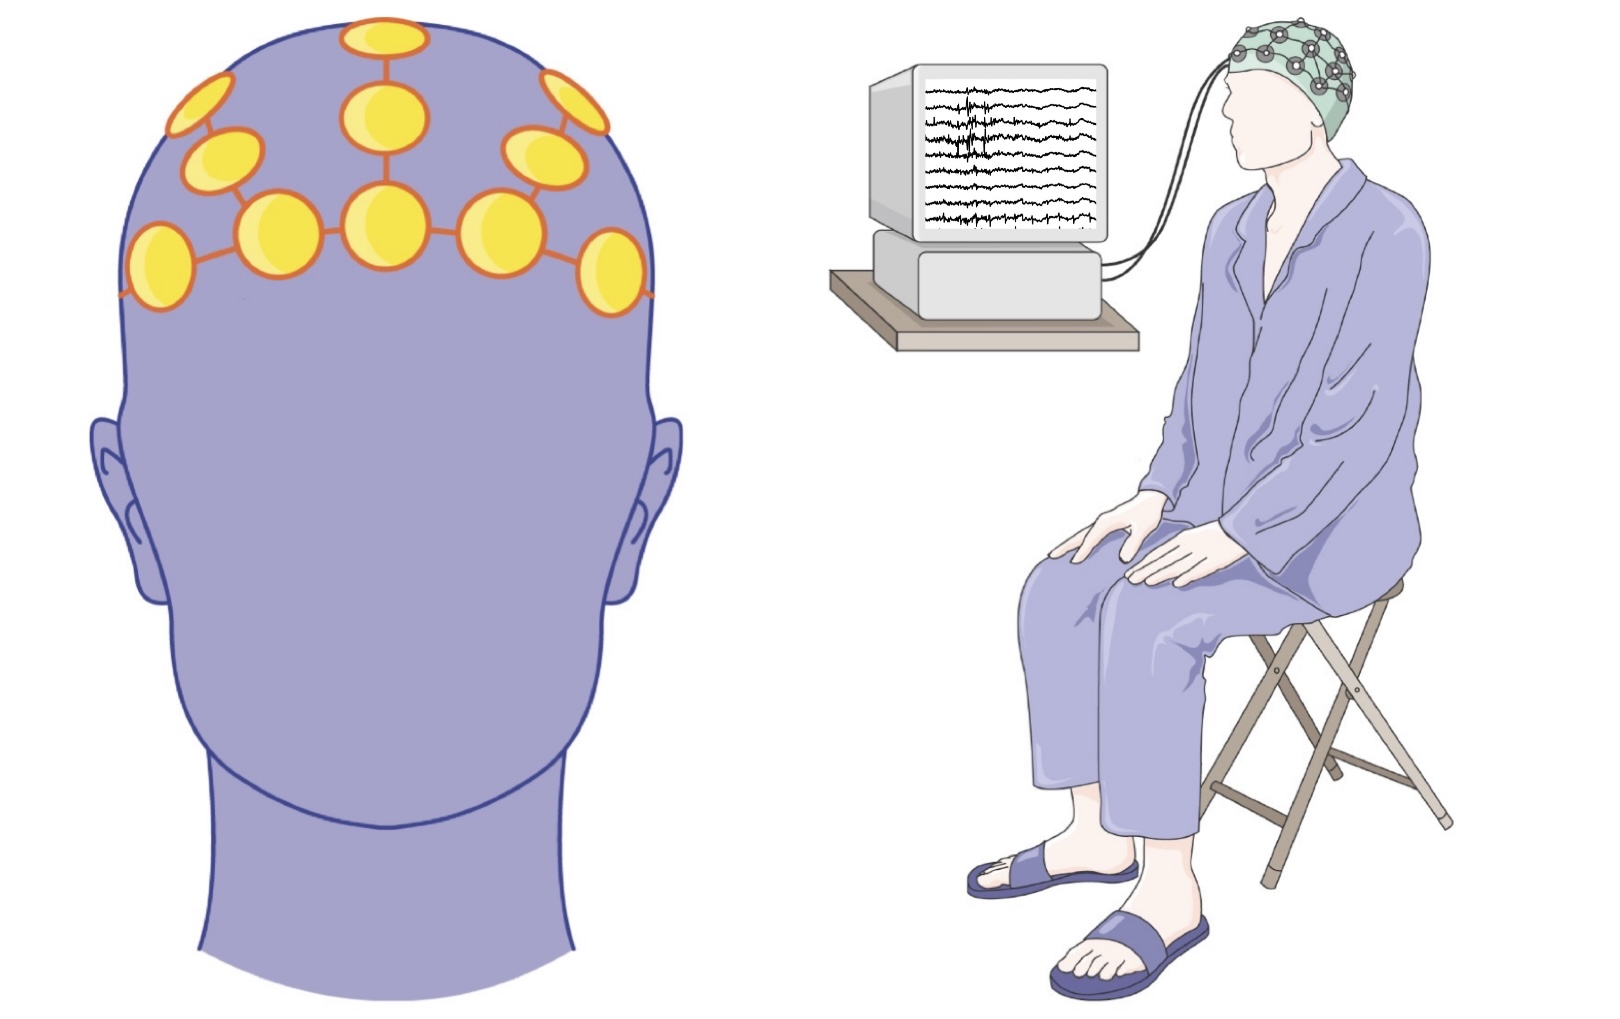
\includegraphics[width=1\textwidth]{figures/new_eeg_wiki.jpg}
    \end{column}
  \end{columns}
\end{frame}



\begin{frame}{What EEG is actually measuring:}
    \begin{itemize}
      \item[$\bullet$] Electrical potentials generated by individual neurons are far too small to be picked up by the recording electrodes.

      \item[$\bullet$] EEG signals are believed to originate from the summation of synchronous activity from thousands of pyramidal neurons with similar spatial orientation.

      \item[$\bullet$] Activity from neurons with different geometric alignments cannot be picked up because their individual electrical signals tend to cancel each other out.

      \item[$\bullet$] Pyramidal neurons are the most frequent type of neuron in the cerebral cortex.

      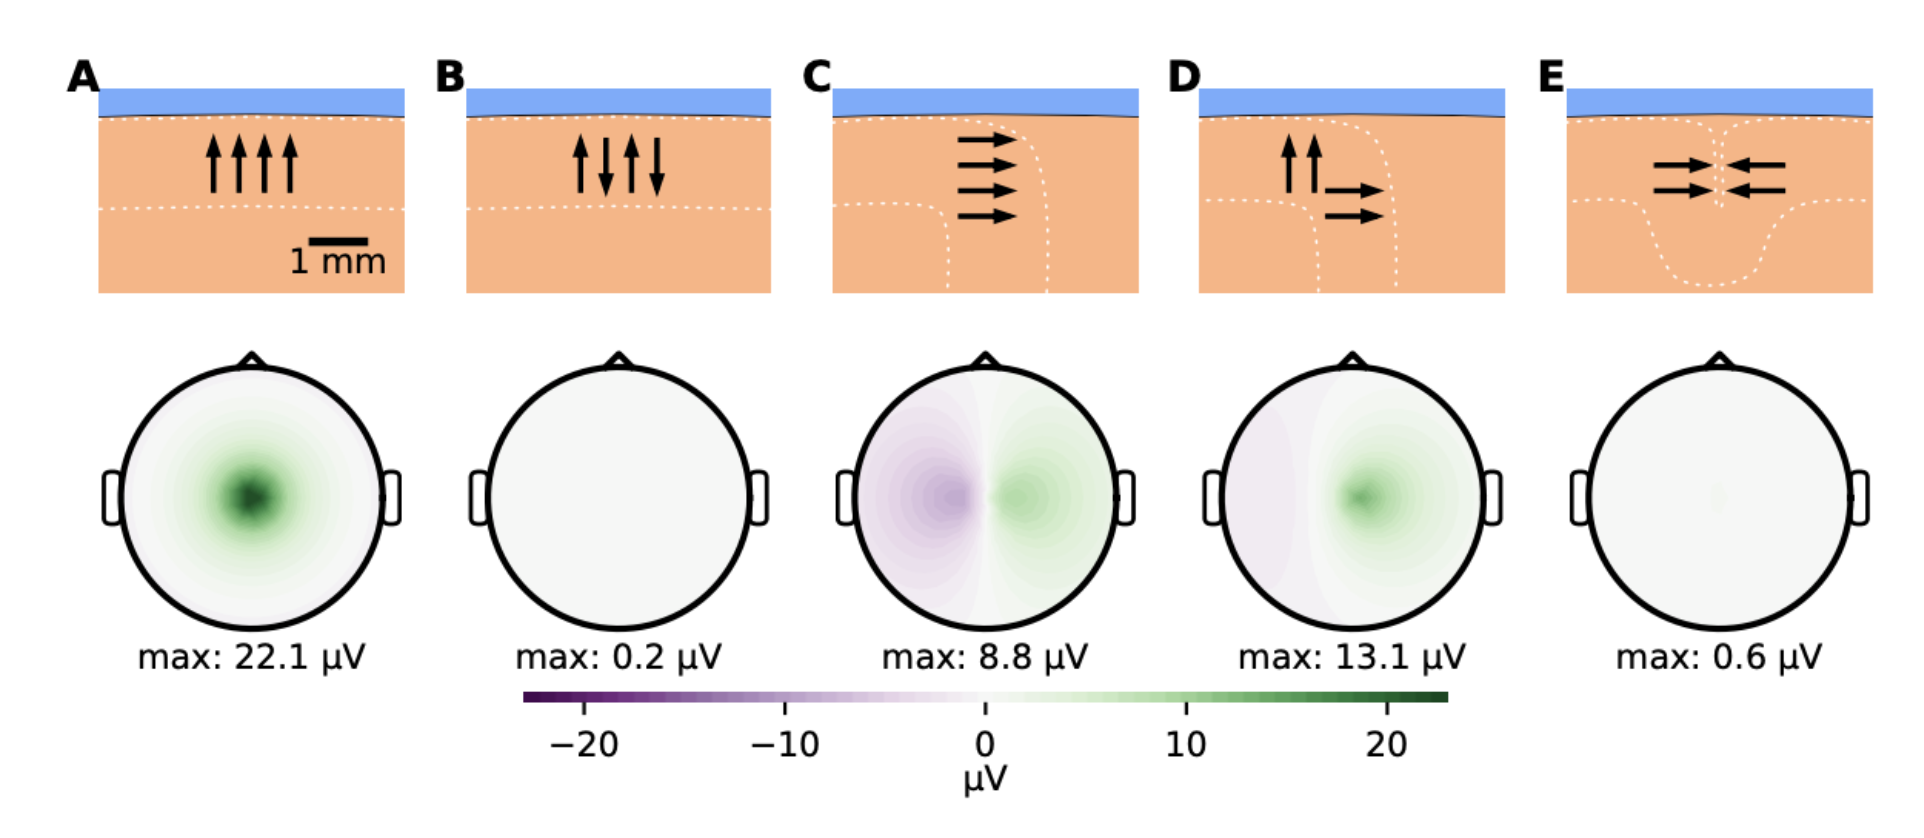
\includegraphics[width=0.5\textwidth]{figures/Dipole_orientation.png}

    \end{itemize}
\end{frame}


%
% \begin{frame}{Current Dipole Approximation I}
%   \begin{itemize}
%     \item[$\bullet$] Extracellular potentials depend on the spatiotemporal distributions of currents over the somatodendric membranes
%     \item[$\bullet$] Membrane currents are commonly referred to as sinks and sources
%     \item[$\bullet$] If we have several point-currents $I_1$, $I_2$, $I_3$..., in locations \textbf{r}$\mathbf{_1}$, \textbf{r}$\mathbf{_2}$,    \textbf{r}$\mathbf{_3}$ ..., the potential in a point	 	\textbf{r} is given by:
%      \begin{equation}
%        \phi(\textbf{r}) = \frac{1}{4\pi\sigma} \sum_{n=1}^N \frac{I_n}{|\textbf{r}-\textbf{r}_n|}
%       \end{equation}
%   \end{itemize}
% \end{frame}

\begin{frame}{Current Dipole Approximation}
  \begin{columns}
    \begin{column}{0.5\textwidth}
      \begin{itemize}
        \item[$\bullet$] Membrane currents are commonly referred to as sinks and sources creating extracellular multipoles
        \item[$\bullet$] If the distance from the center of a volume containing a set of current sources to the measurement point is larger than the maximal distance from volume center to any source, the extracellular potential can be written as following through the use of multipole expansion:
          \begin{equation}
            \phi(R) = \frac{C_\text{monopole}}{R} + \frac{C_\text{dipole}}{R^2} + \frac{C_\text{quadrupole}}{R^3} + \frac{C_\text{octopole}}{R^4} + \ldots
          \end{equation}
        \item[$\bullet$] Net sum of currents over neuronal membrane is always zero, thus $C_\text{monopole} = 0$.
        \item[$\bullet$] Quadrupole, octupole and higher-order contributions decay rapidly with distance $R$.
        % \item[$\bullet$] For large distances, such as in EEG, the potential can be approximated by the dipole contribution:
        %   \begin{equation}
        %     \phi(R) \approx \frac{C_\text{dipole}}{R^2} = \frac{1}{4\pi\sigma}\frac{|\textbf{p}| \text{cos} \theta}{\lvert\textbf{r}-\textbf{r}_p\rvert^2}.
        %   \end{equation}
      \end{itemize}
    \end{column}
    \begin{column}{0.5\textwidth}
      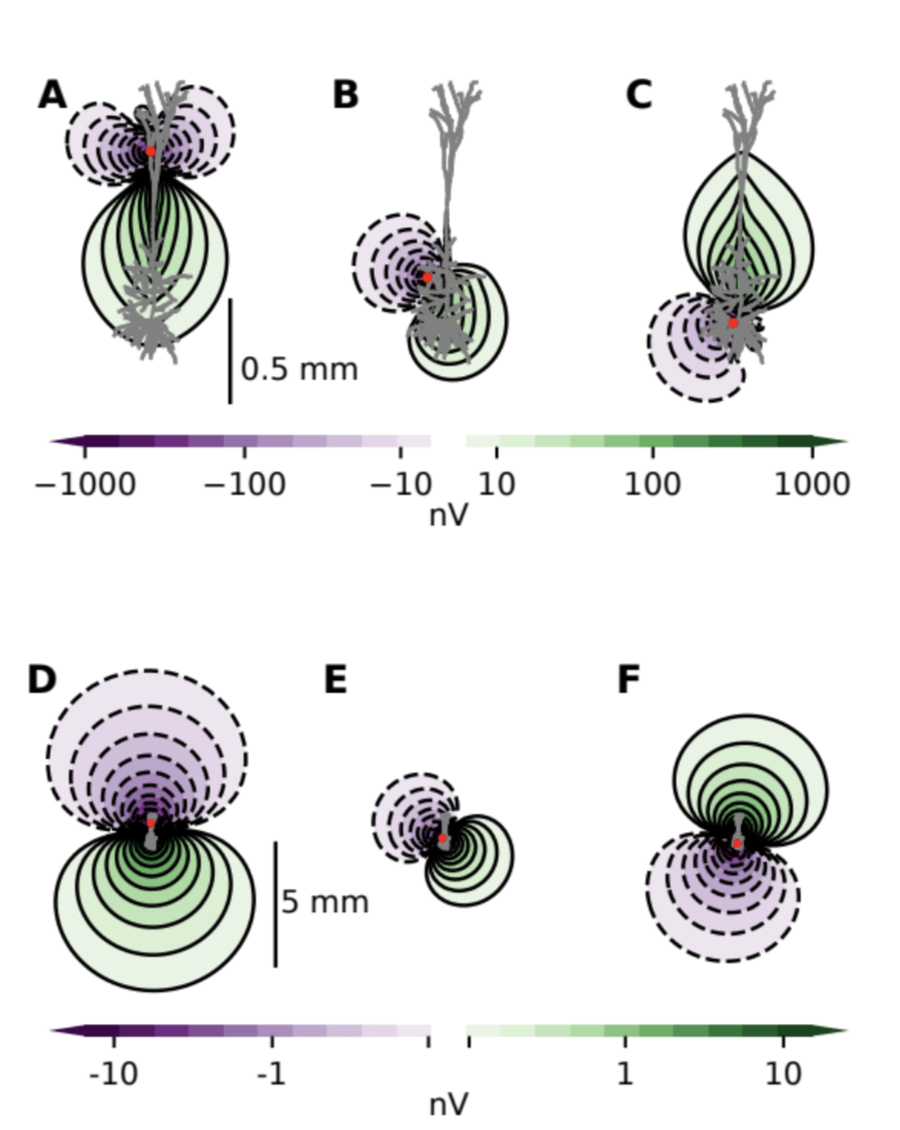
\includegraphics[width=0.7\textwidth]{figures/dipole_pattern.png}
    \end{column}
  \end{columns}
\end{frame}



\begin{frame}{The New York Head Model & LFPy}
    \begin{itemize}
        \item[$\bullet$] Highly detailed computer model designed for simulating electrical brain activity
        \item[$\bullet$] Based on MRI data from 152 adult heads
        \item[$\bullet$] Scalp, skull, cerebrospinal fluid, gray matter, white matter and cavities
        \item[$\bullet$] Precise information about tissue geometry and electrical properties
        \item[$\bullet$] Lead field $L$ links the sensitivity of EEG measurements from various scalp locations to potential neural current source locations
        \item[$\bullet$] $L$ is computed for 74,382 discrete points in cortex with 231 electrode positions on the scalp
        \item[$\bullet$] The forward modelling of the EEG signal $\phi$ can be described through:
          \begin{equation}
            \phi = L\textbf{p}
          \end{equation}
        \item[$\bullet$] The NYHM is integrated into LFPy - a tool for calculating EEG signals from biophysically detailed neural simulations
    \end{itemize}
\end{frame}


\begin{frame}[fragile]{Calculating EEG signals}
    \begin{columns}
        \begin{column}{0.5\textwidth}
            \begin{itemize}
                \item[$\bullet$] To sample a single data point we position a current dipole moment at one of the possible locations, and calculate its corresponding EEG signal
                \item[$\bullet$] Dipole magnitude is set to 1 nAm
                {\scriptsize
                \begin{verbatim}
    def calculate_eeg(nyhead, A: float = 1.0):
        """
        Calculates the eeg signal from the dipole population

        returns:
            eeg_i : array of length (231)
        """
        L = nyhead.get_transformation_matrix()

        # Static dipole without temporal axis
        p = np.array(([0.0], [0.0], [A])) * 1E7  # [nA* mu m]

        # Rotates the direction of the dipole moment
        # so that it is normal to the cerebral cortex
        p = nyhead.rotate_dipole_to_surface_normal(p)

        # Generates the EEG signal originating from the dipole moment
        eeg_i = L @ p * 1E3 # [mV]

        return eeg_i.ravel()
                \end{verbatim}
                }
            \end{itemize}
        \end{column}
        \begin{column}{0.5\textwidth}
          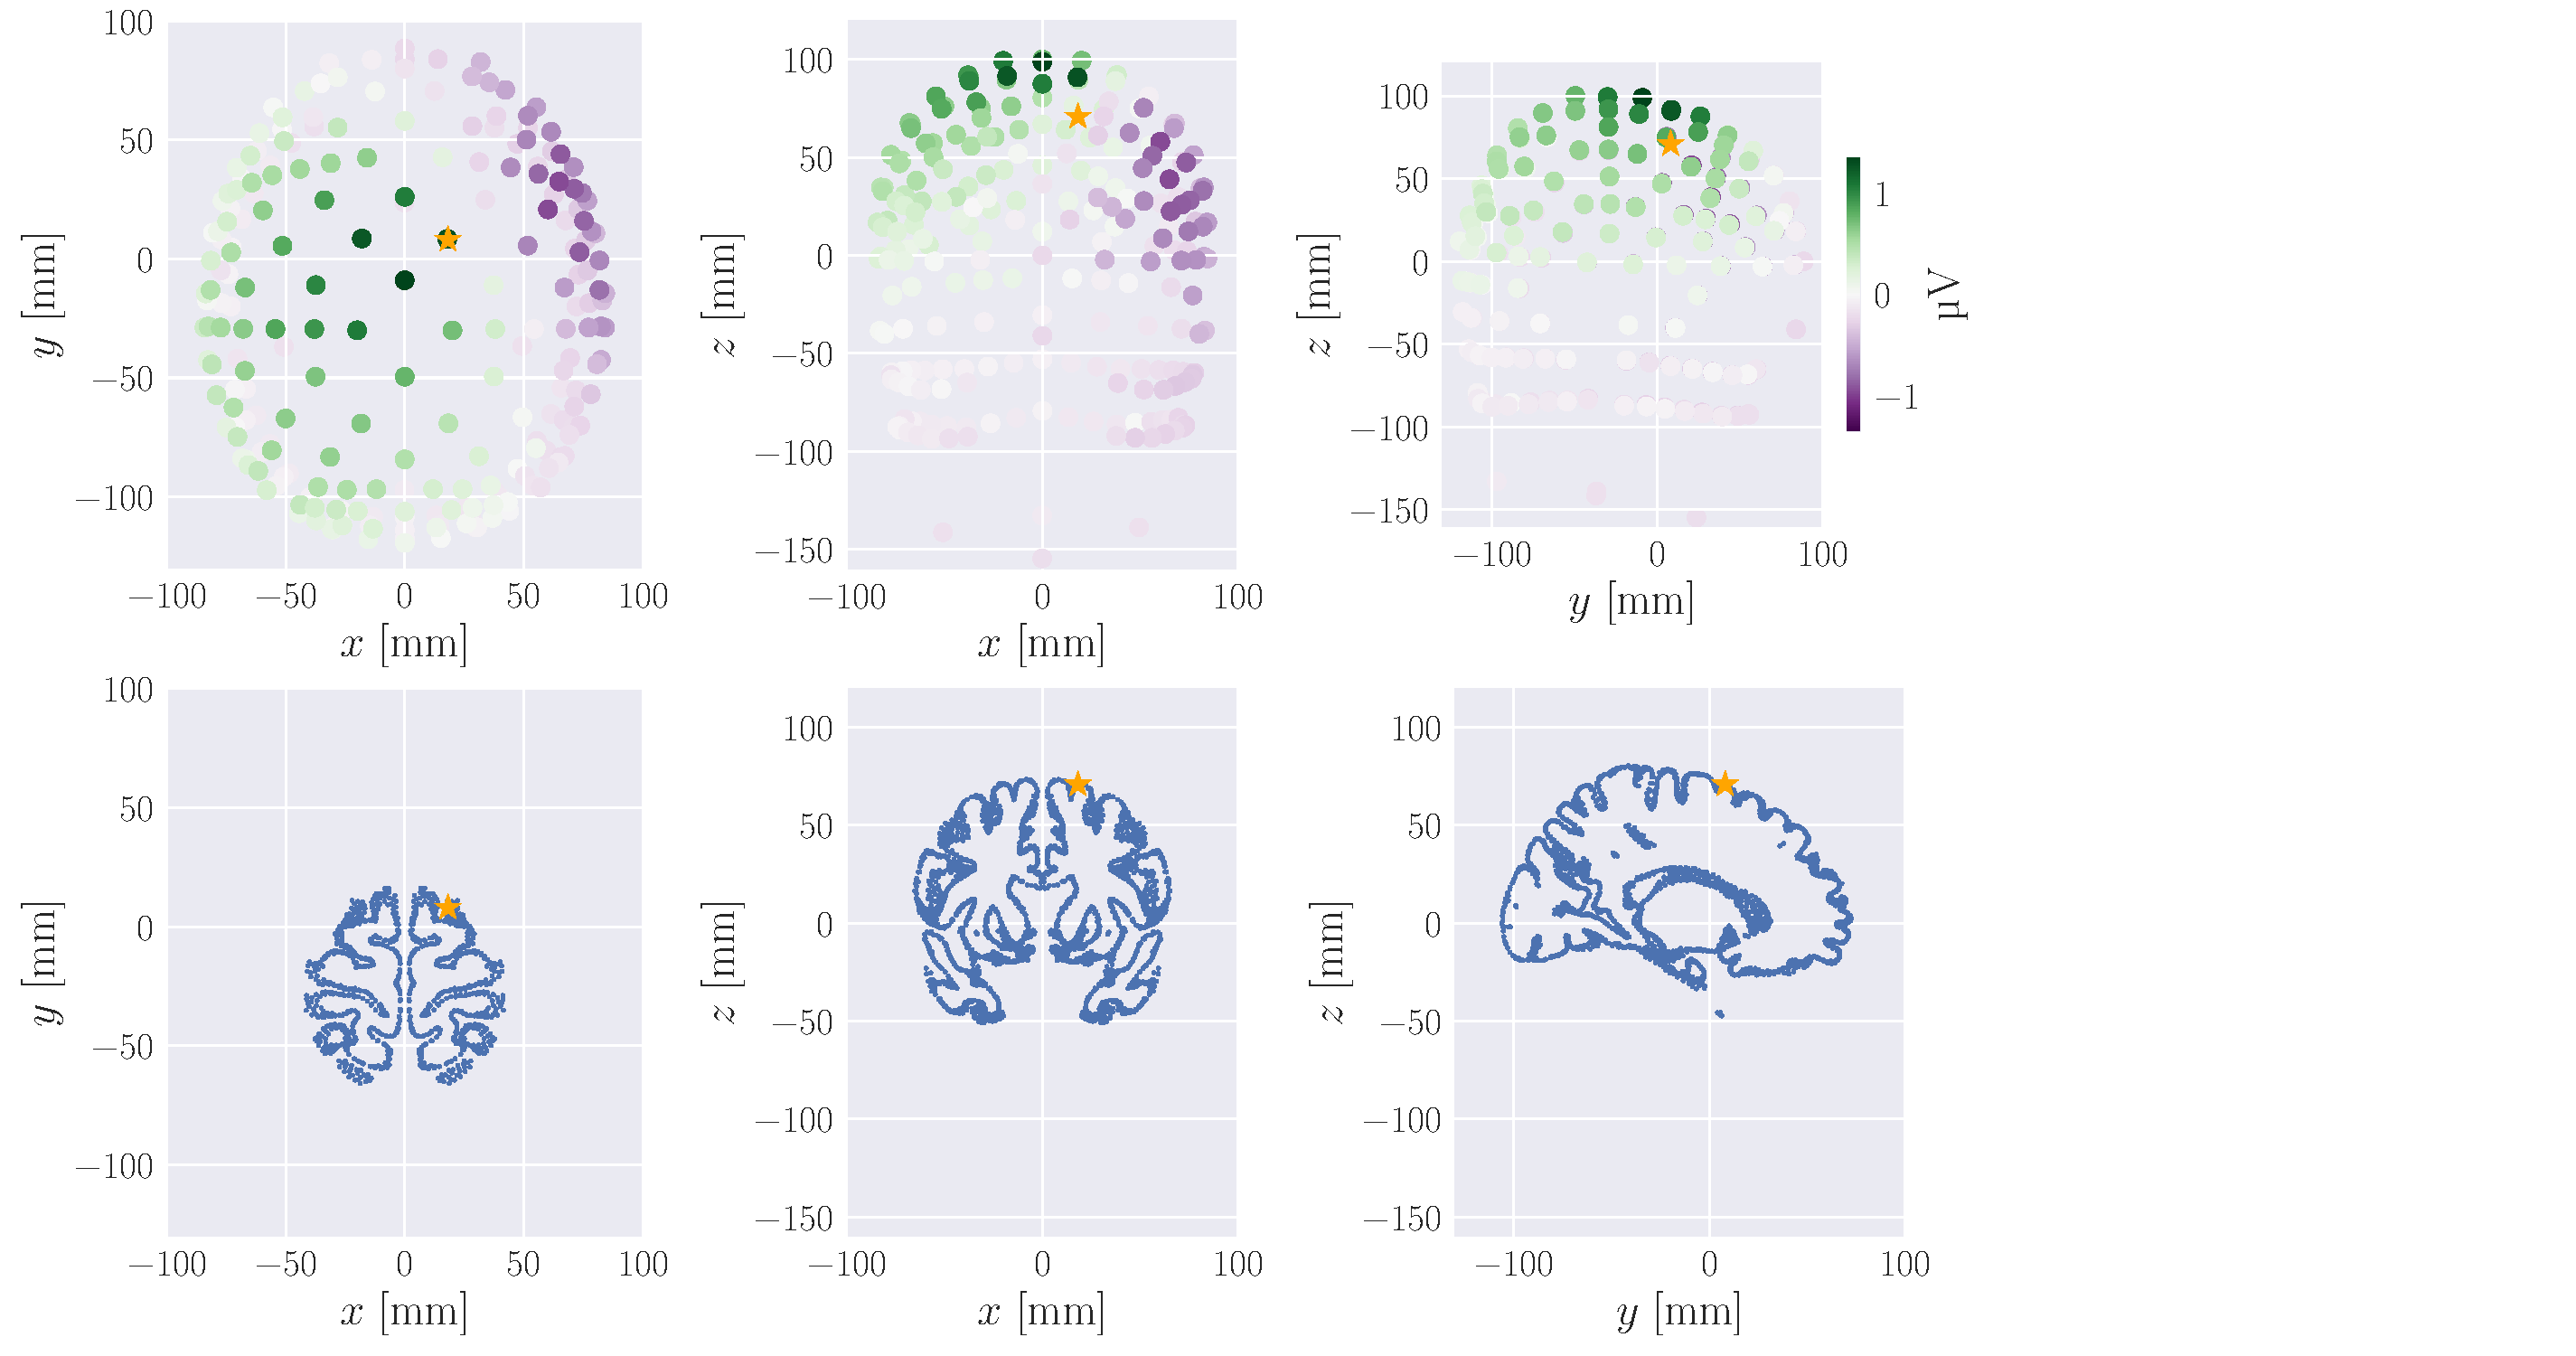
\includegraphics[width=1.0\textwidth]{figures/simple_example.pdf}
        \end{column}
    \end{columns}
\end{frame}


\begin{frame}{Final Data Set}
  \begin{columns}
    \begin{column}{0.5\textwidth}
      \begin{itemize}
        \item[$\bullet$] To align with real-world EEG samples, controlled noise is intentionally introduced to the data.
        \item[$\bullet$] Normally distributed noise with mean of 0 and standard deviation equal to 10$\%$ of the standard deviation observed in the simulated EEG recordings.
        \item[$\bullet$] 70,000 samples, where each sample holds 231 values representing the EEG measurements recorded at each electrode
        \item[$\bullet$] Target values for the EEG samples are the $x$-, $y$- and $z$-coordinates of the different dipole sources.
        % \item[$\bullet$] We sample the EEG data to obtain what we may consider ERPs, holding a specific time step within a EEG time series where an averaged signal attains its maximum magnitude, resulting in a "static" EEG signal
        % \item[$\bullet$] Time-locked, one-dimensional EEG signals capturing the instantaneously dipole activity within the brain
      \end{itemize}
    \end{column}
    \begin{column}{0.5\textwidth}
      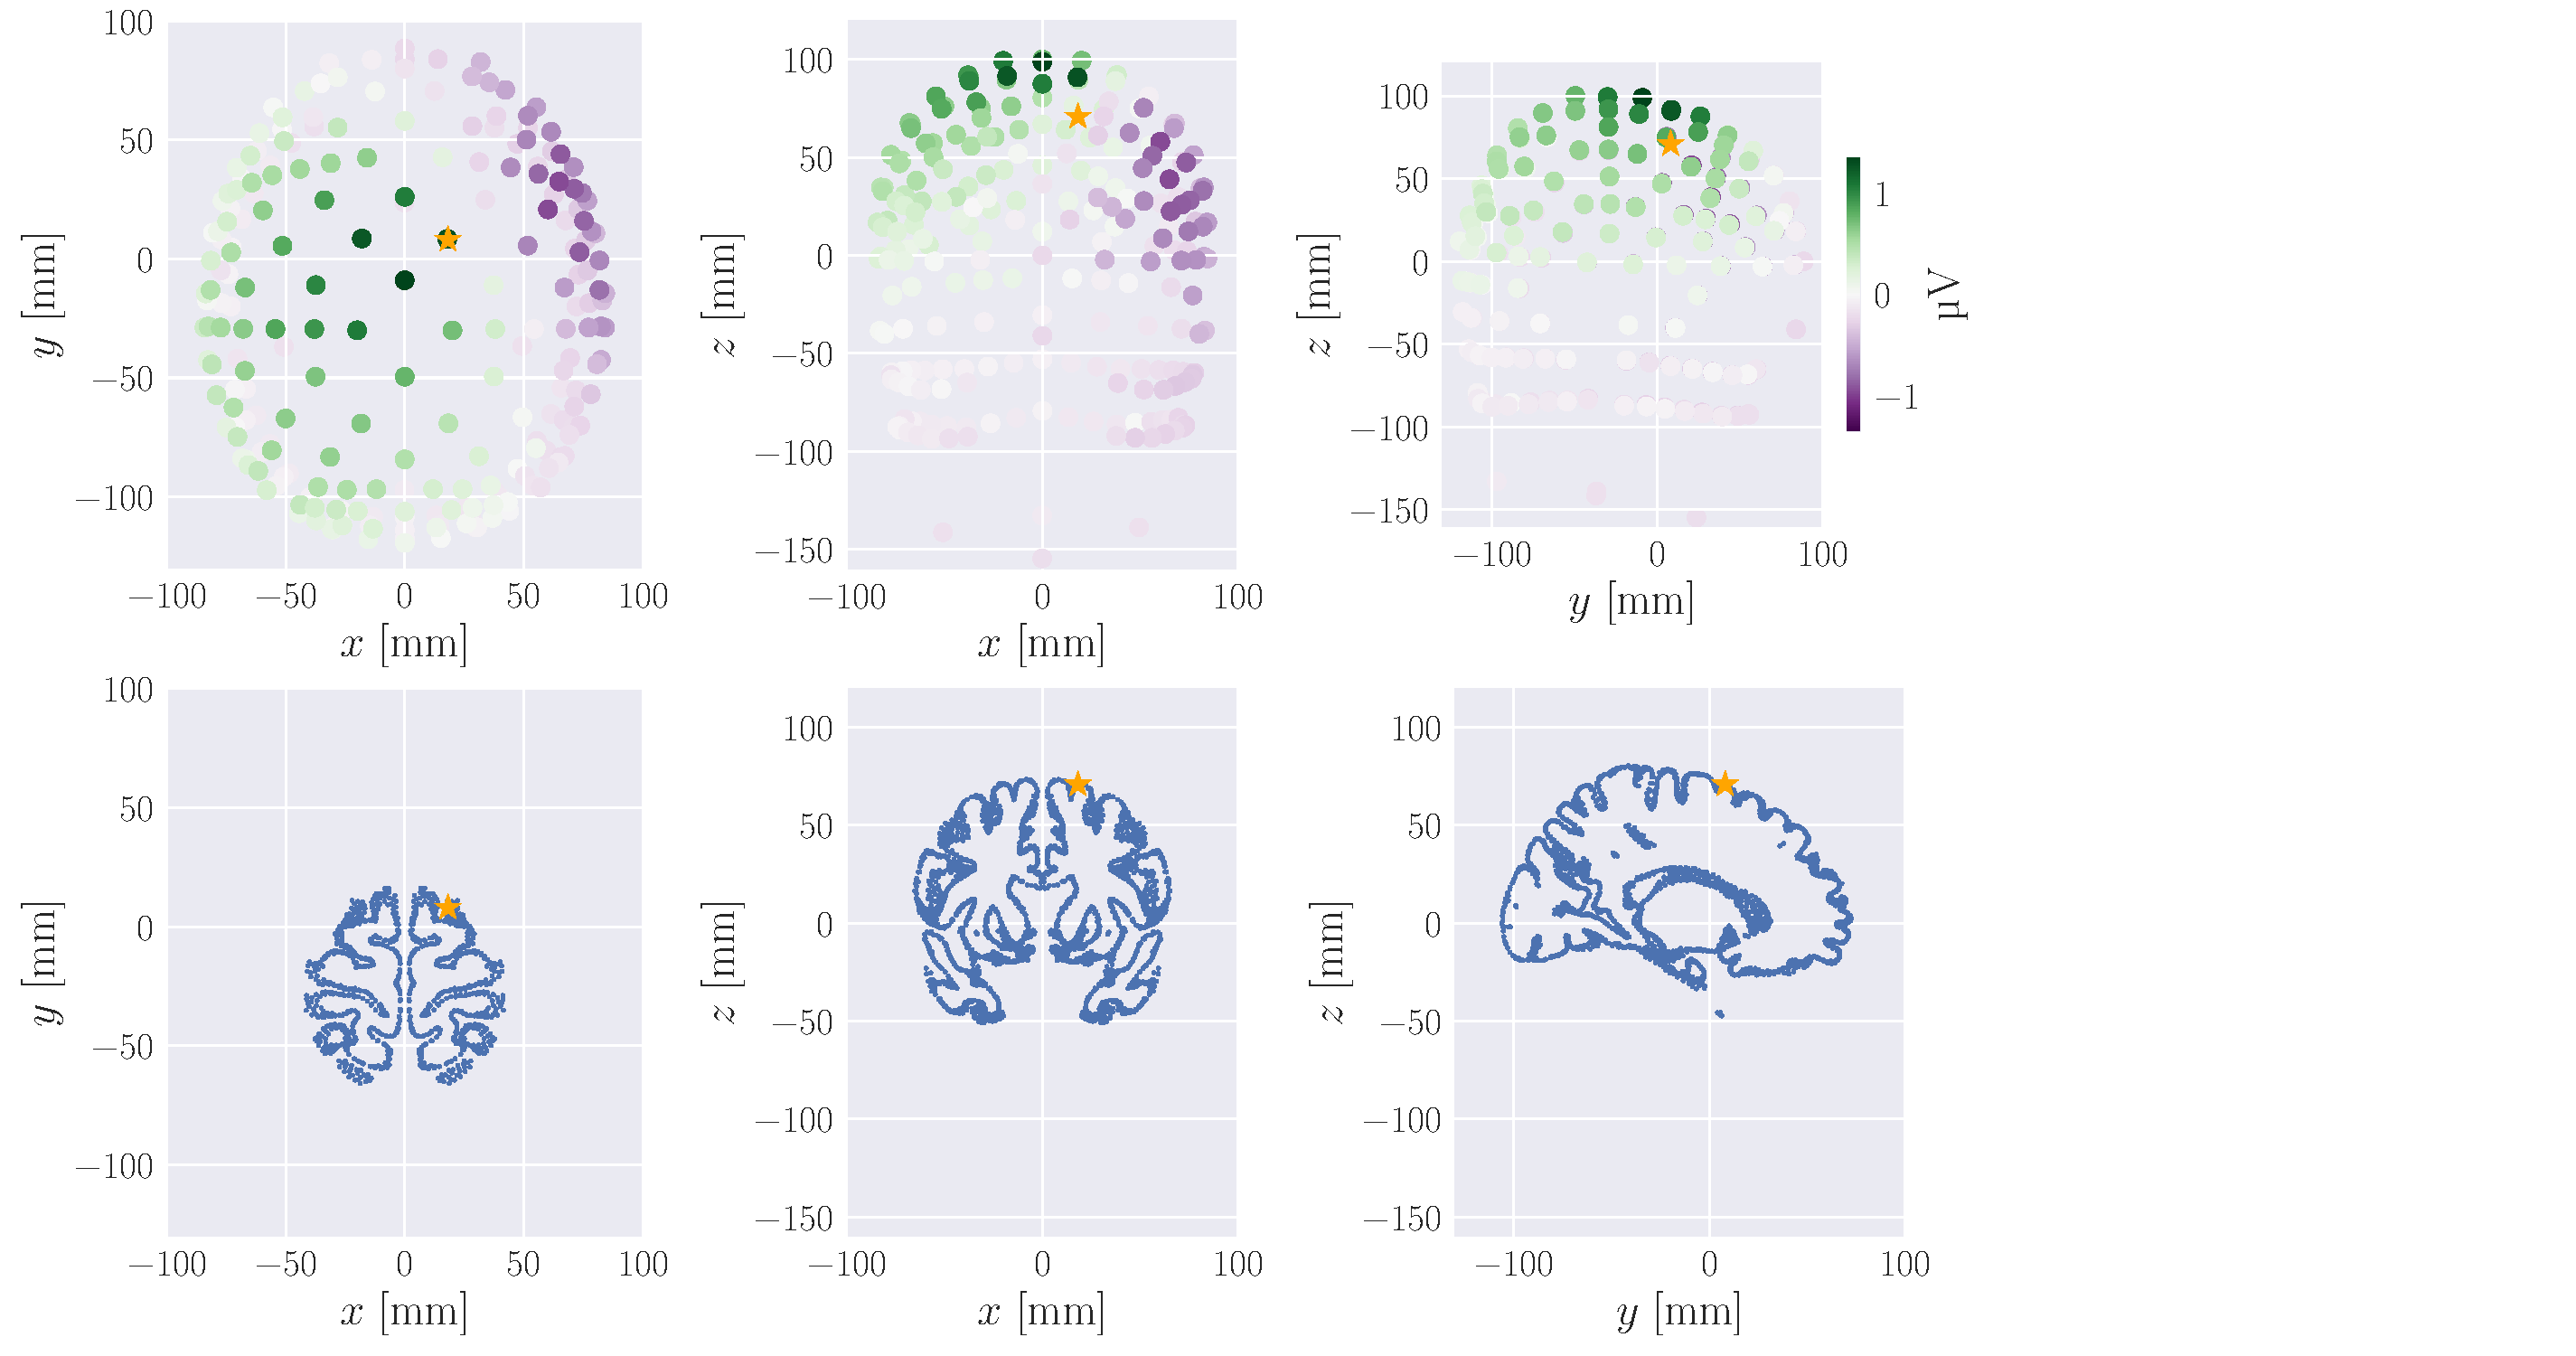
\includegraphics[width=1.0\textwidth]{figures/simple_example.pdf}
    \end{column}
  \end{columns}
\end{frame}

% \begin{frame}{Interpretation of the Data}
%     \begin{itemize}
%         \item[$\bullet$] A widely recognized method for EEG investigation involves the practice of averaging EEG responses to specific stimuli across multiple trials
%         \item[$\bullet$] These temporally aligned segments of EEG signals are commonly referred to as event-related potentials (ERPs)
%         \item[$\bullet$] This technique facilitates the identification of the specific time step within the EEG time series where the averaged signal attains its maximum magnitude, resulting in a "static" EEG signal characterized by reduced noise.
%         \item[$\bullet$] We sample the EEG data to obtain what we may consider an ERP, representing a static snapshot of the electrode recordings of a current dipole source
%         \item[$\bullet$] Time-locked, one-dimensional EEG signals capturing the instantaneously dipole activity within the brain
%     \end{itemize}
% \end{frame}


\begin{frame}{Building a FCNN}
  \begin{columns}
    \begin{column}{0.5\textwidth}
      \begin{itemize}
        \item[$\bullet$] Neural Networks mimics the way biological neurons transmit signals, with interconnected nodes that communicate through mathematical functions.
        \item[$\bullet$] FCNN: outputs is only sent forward through all of the layers.
        \item[$\bullet$] Neurons are connected with trainable weights, representing connection strengths.
        \item[$\bullet$] Each neuron holds individual biases that are added to the weighted sum and increase model flexibility.
        \item[$\bullet$] Activation funcrions are applied to each neuron's output and introduce non-linearity for learning complex data patterns.
    \end{itemize}
    \end{column}
    \begin{column}{0.5\textwidth}
      \begin{itemize}
        % \item[$\bullet$] Architecture is determined by trial-and-error
      \item[$\bullet$] 300,000 trainable parameters
      \item[$\bullet$] ReLU in input layer: $f(x) = \max(0, x)$
      \item[$\bullet$] Tanh in hidden layers: $f(x) = \tanh(x)$
      \end{itemize}
      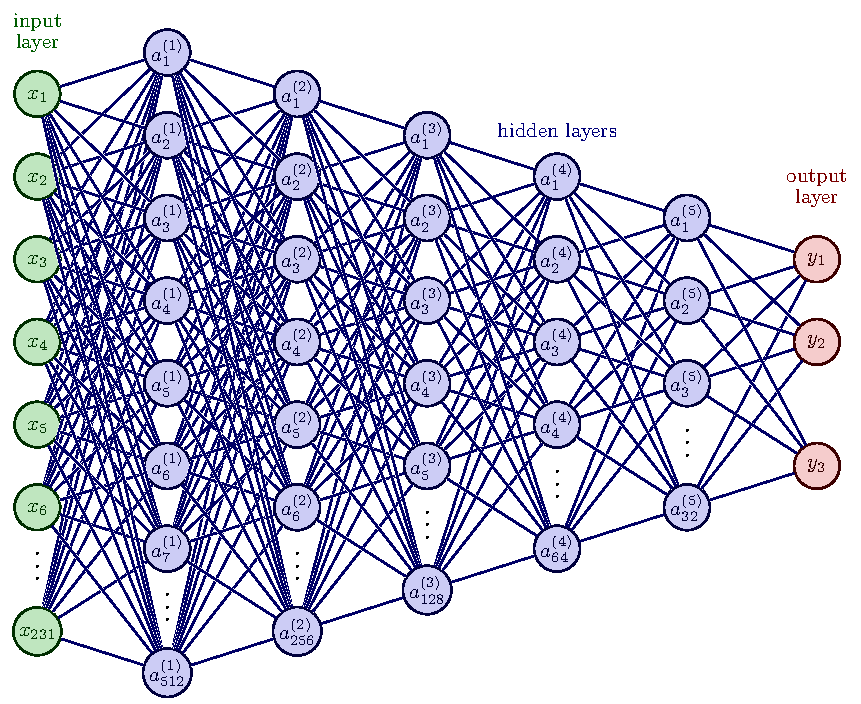
\includegraphics[width=1.0\textwidth]{figures/FFNN_architecture.pdf}
    \end{column}
  \end{columns}
\end{frame}

\begin{frame}{Training the Network}
    \begin{itemize}
      \item[$\bullet$] Data segmentation: \emph{Training Set}, \emph{Validation Set}, \emph{Test Set}
      % \item[$\bullet$] Centering the EEG data around the mean and scaling it to achieve unit standard deviation
      \item[$\bullet$] To evaluate how well the model make predictions, Loss Function:
      \begin{equation}
        \text{MED}(\boldsymbol{\theta})
          = \frac{1}{N} \sum_{i=1}^{N}
              \sqrt{(x_i - \tilde{x}_i)^2 + (y_i - \tilde{y}_i)^2 + (z_i - \tilde{z}_i)^2}.
      \end{equation}
      \item[$\bullet$] Backpropagation for calculating the gradients of the loss function with respect to each parameter in the network.
      \item[$\bullet$] Gradient Descent (with momentum) uses the gradients to iteratively update the parameters. It adjusts the parameters in the direction opposite to the gradient of the loss function -- a process that continues until a minimum of the loss function is reached.
    \end{itemize}
\end{frame}

% \begin{frame}{Objectives}
%     \begin{itemize}
%       \item[$\bullet$] Source localization using spherical head models typically yields localization errors in the range of 10-30 mm (Akalin and Makeig 2013, Biasiucci et al. 2019).
%       \item[$\bullet$] Modern subject-specific head models is expected to result in mean Euclidean errors less than 10 mm (Akalin and Makeig 2013, Biasiucci et al. 2019).
%       \item[$\bullet$] Primary objective is to ascertain whether a simple fully connected feed-forward neural network can effectively discern patterns and approximate dipole positions within this threshold.
%     \end{itemize}
% \end{frame}


\begin{frame}{Localizing Single Current Dipole Sources}
  \begin{columns}
    \begin{column}{0.5\textwidth}
      \begin{itemize}
        \item[$\bullet$] Training time of 1.5 hours, 500 epochs
        % \item[$\bullet$] Training loss = 0.317 mm
        \item[$\bullet$] Validation loss = 1.781 mm.
        \item[$\bullet$] Test loss = 1.33 mm
    \end{itemize}
    % \begin{table}[]
    %   \centering
    % \begin{tabular}{|ccc|}
    % \hline
    % \rowcolor[HTML]{CBCEFB}
    % \multicolumn{3}{|c|}{\cellcolor[HTML]{CBCEFB}\textbf{Euclidean Distance for Test Samples}}                                                             \\ \hline
    % \rowcolor[HTML]{EFEFEF}
    % \multicolumn{1}{|c|}{\cellcolor[HTML]{EFEFEF}ED \textless 5 mm} & \multicolumn{1}{c|}{\cellcolor[HTML]{EFEFEF}ED \textless 10 mm} & ED \textless 15 mm \\ \hline
    % \rowcolor[HTML]{FFFFFF}
    % \multicolumn{1}{|c|}{\cellcolor[HTML]{FFFFFF}99.735 $\%$}       & \multicolumn{1}{c|}{\cellcolor[HTML]{FFFFFF}99.995 $\%$}        & 100$\%$        \\ \hline
    % \end{tabular}
    % \end{table}
    \end{column}

    \begin{column}{0.5\textwidth}
      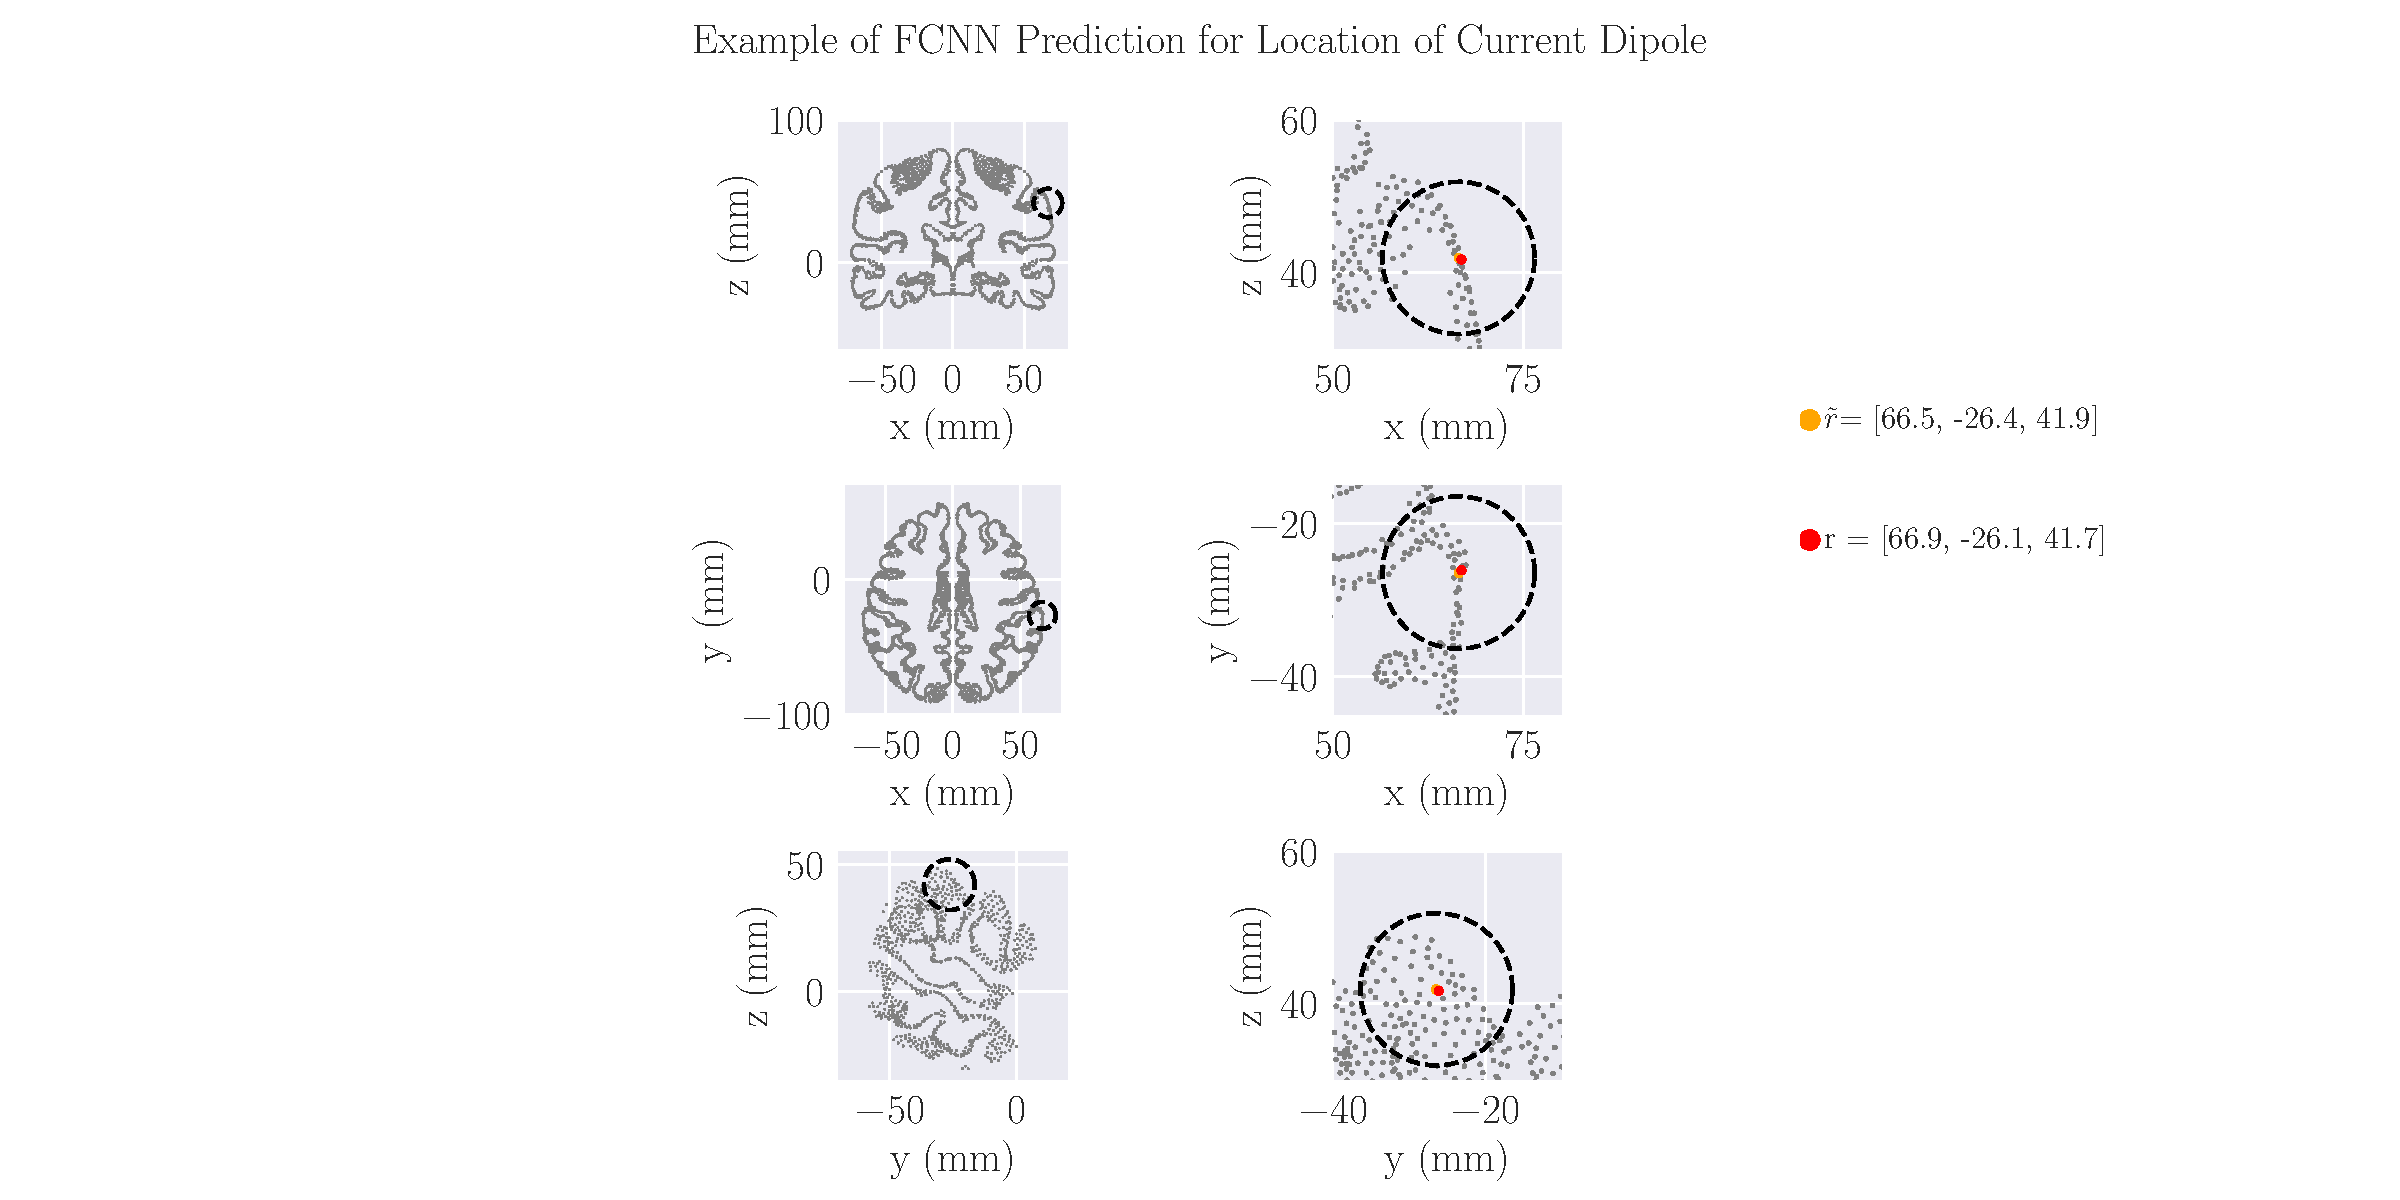
\includegraphics[width=1.0\textwidth]{figures/FFNN_single_dipole_prediction.pdf}
      \item[$\bullet$] Euclidean distance = 0.54 mm
    \end{column}

  \end{columns}
\end{frame}


% \begin{frame}{Localizing Single Current Dipole Sources II}
%   \begin{columns}
%     \begin{column}{0.3\textwidth}
%       \begin{itemize}
%         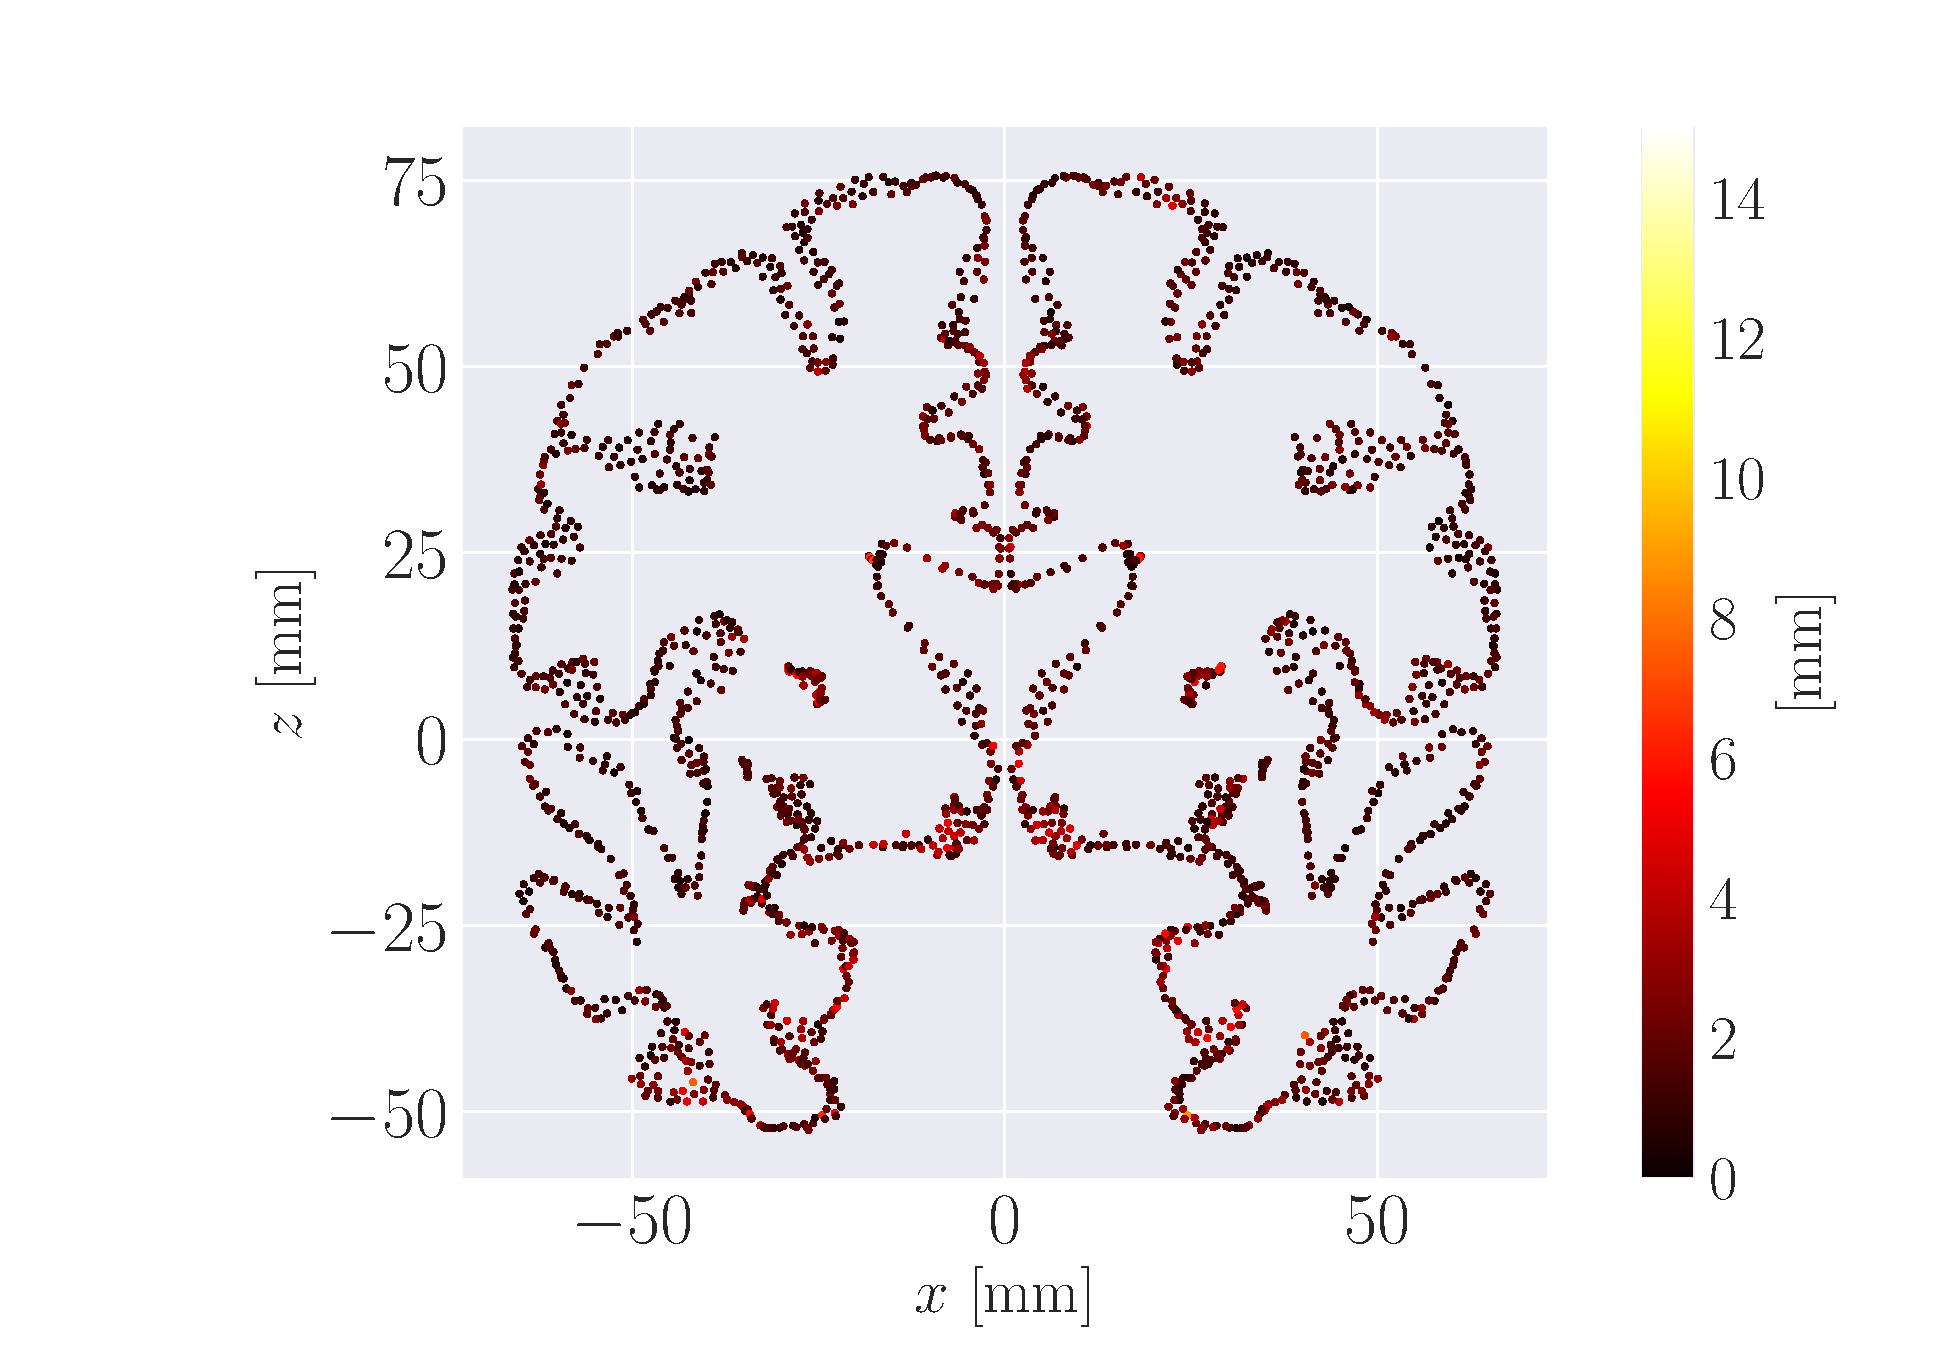
\includegraphics[width=1.0\textwidth]{figures/MED_simple_dipole_error_Euclidean Distance_0.pdf}
%       \end{itemize}
%     \end{column}
%     \begin{column}{0.3\textwidth}
%       \begin{itemize}
%         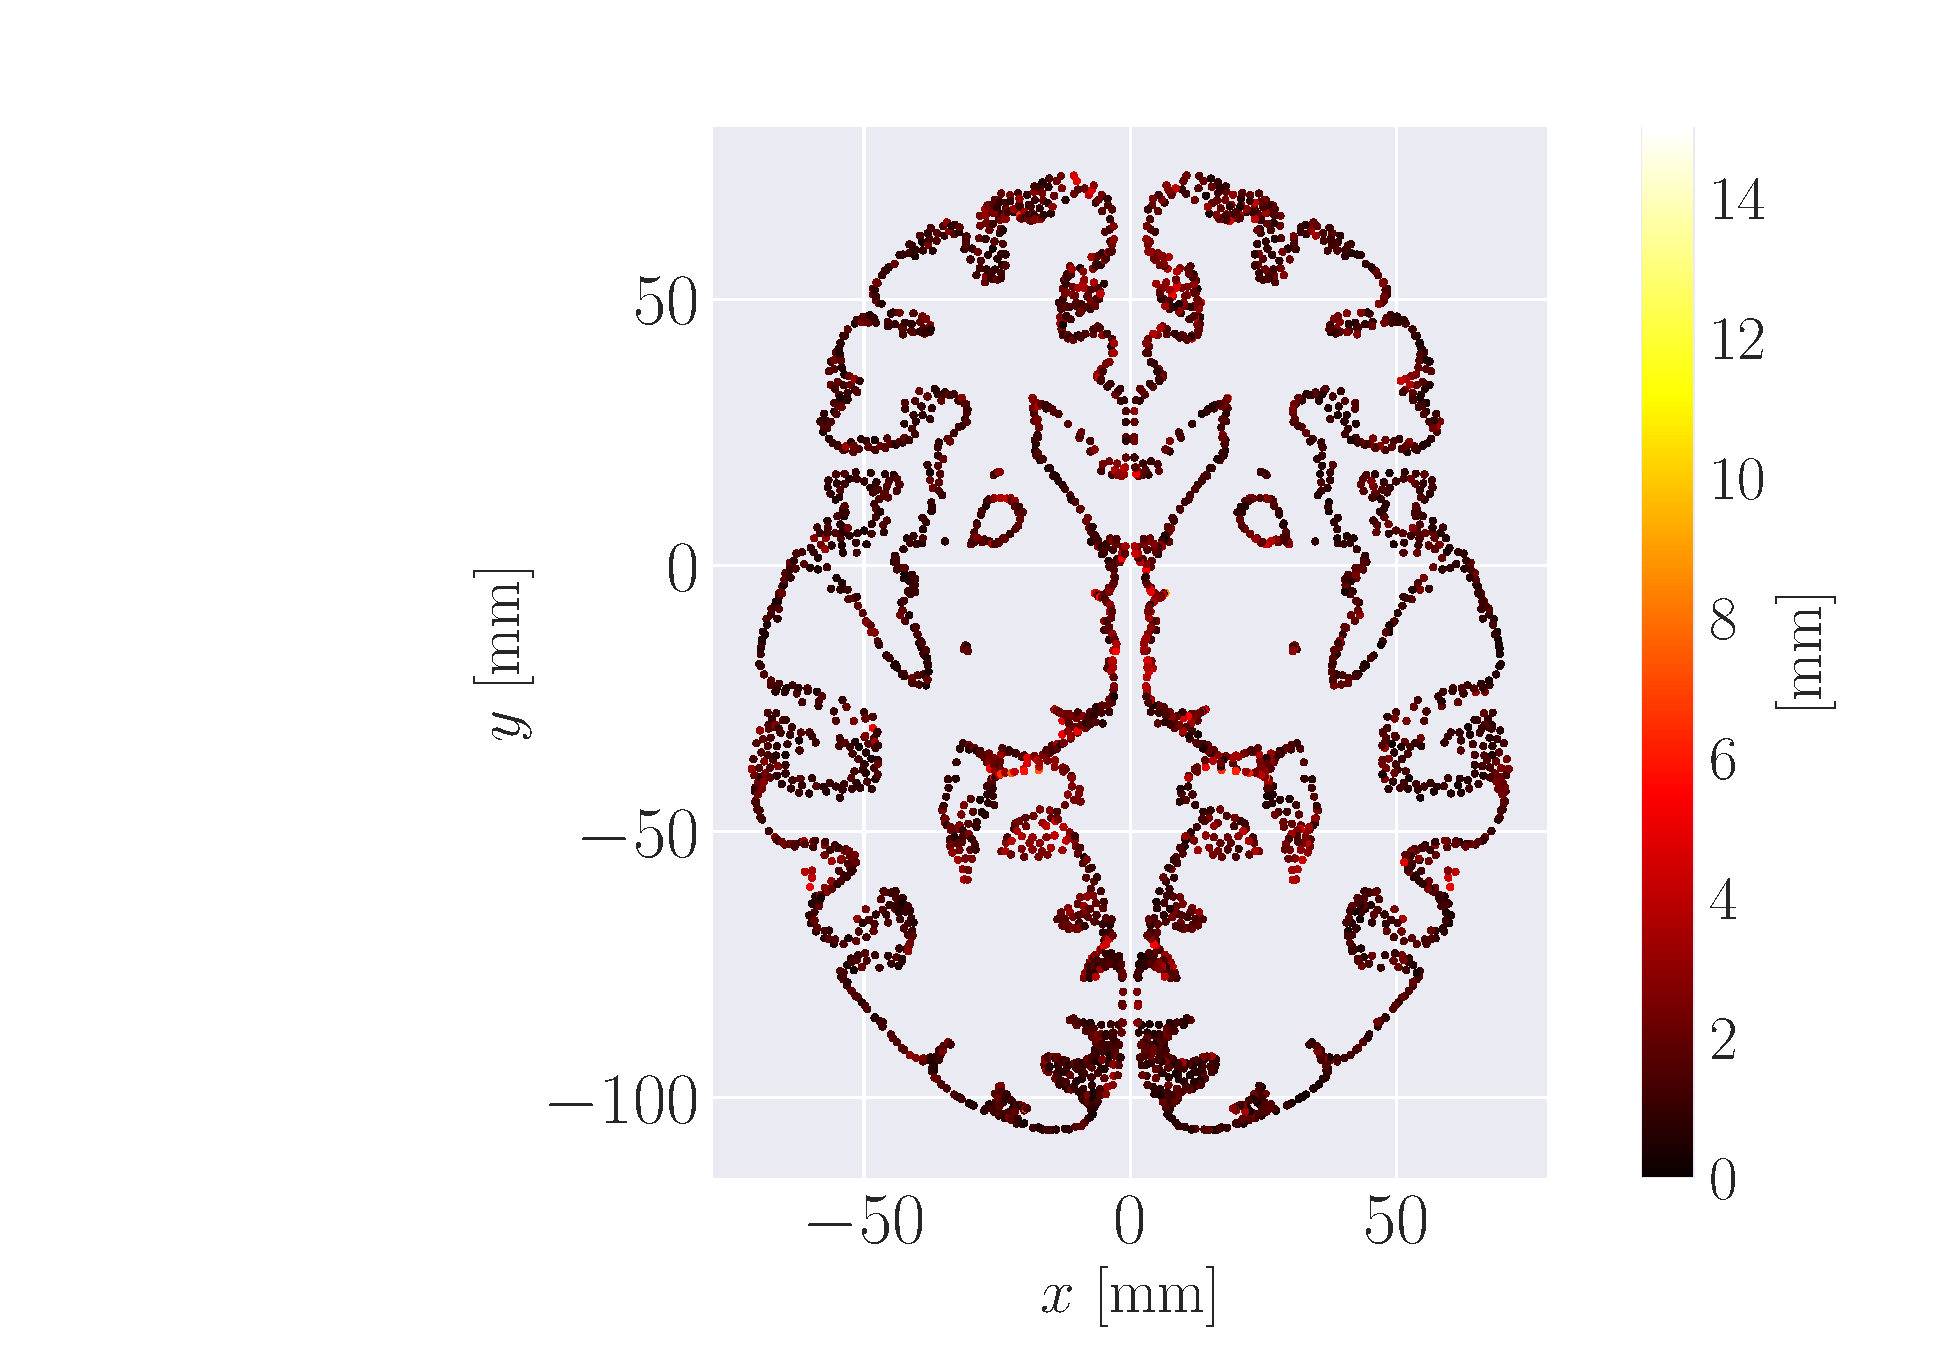
\includegraphics[width=1.0\textwidth]{figures/MED_simple_dipole_error_Euclidean Distance_1.pdf}
%       \end{itemize}
%     \end{column}
%     \begin{column}{0.3\textwidth}
%       \begin{itemize}
%         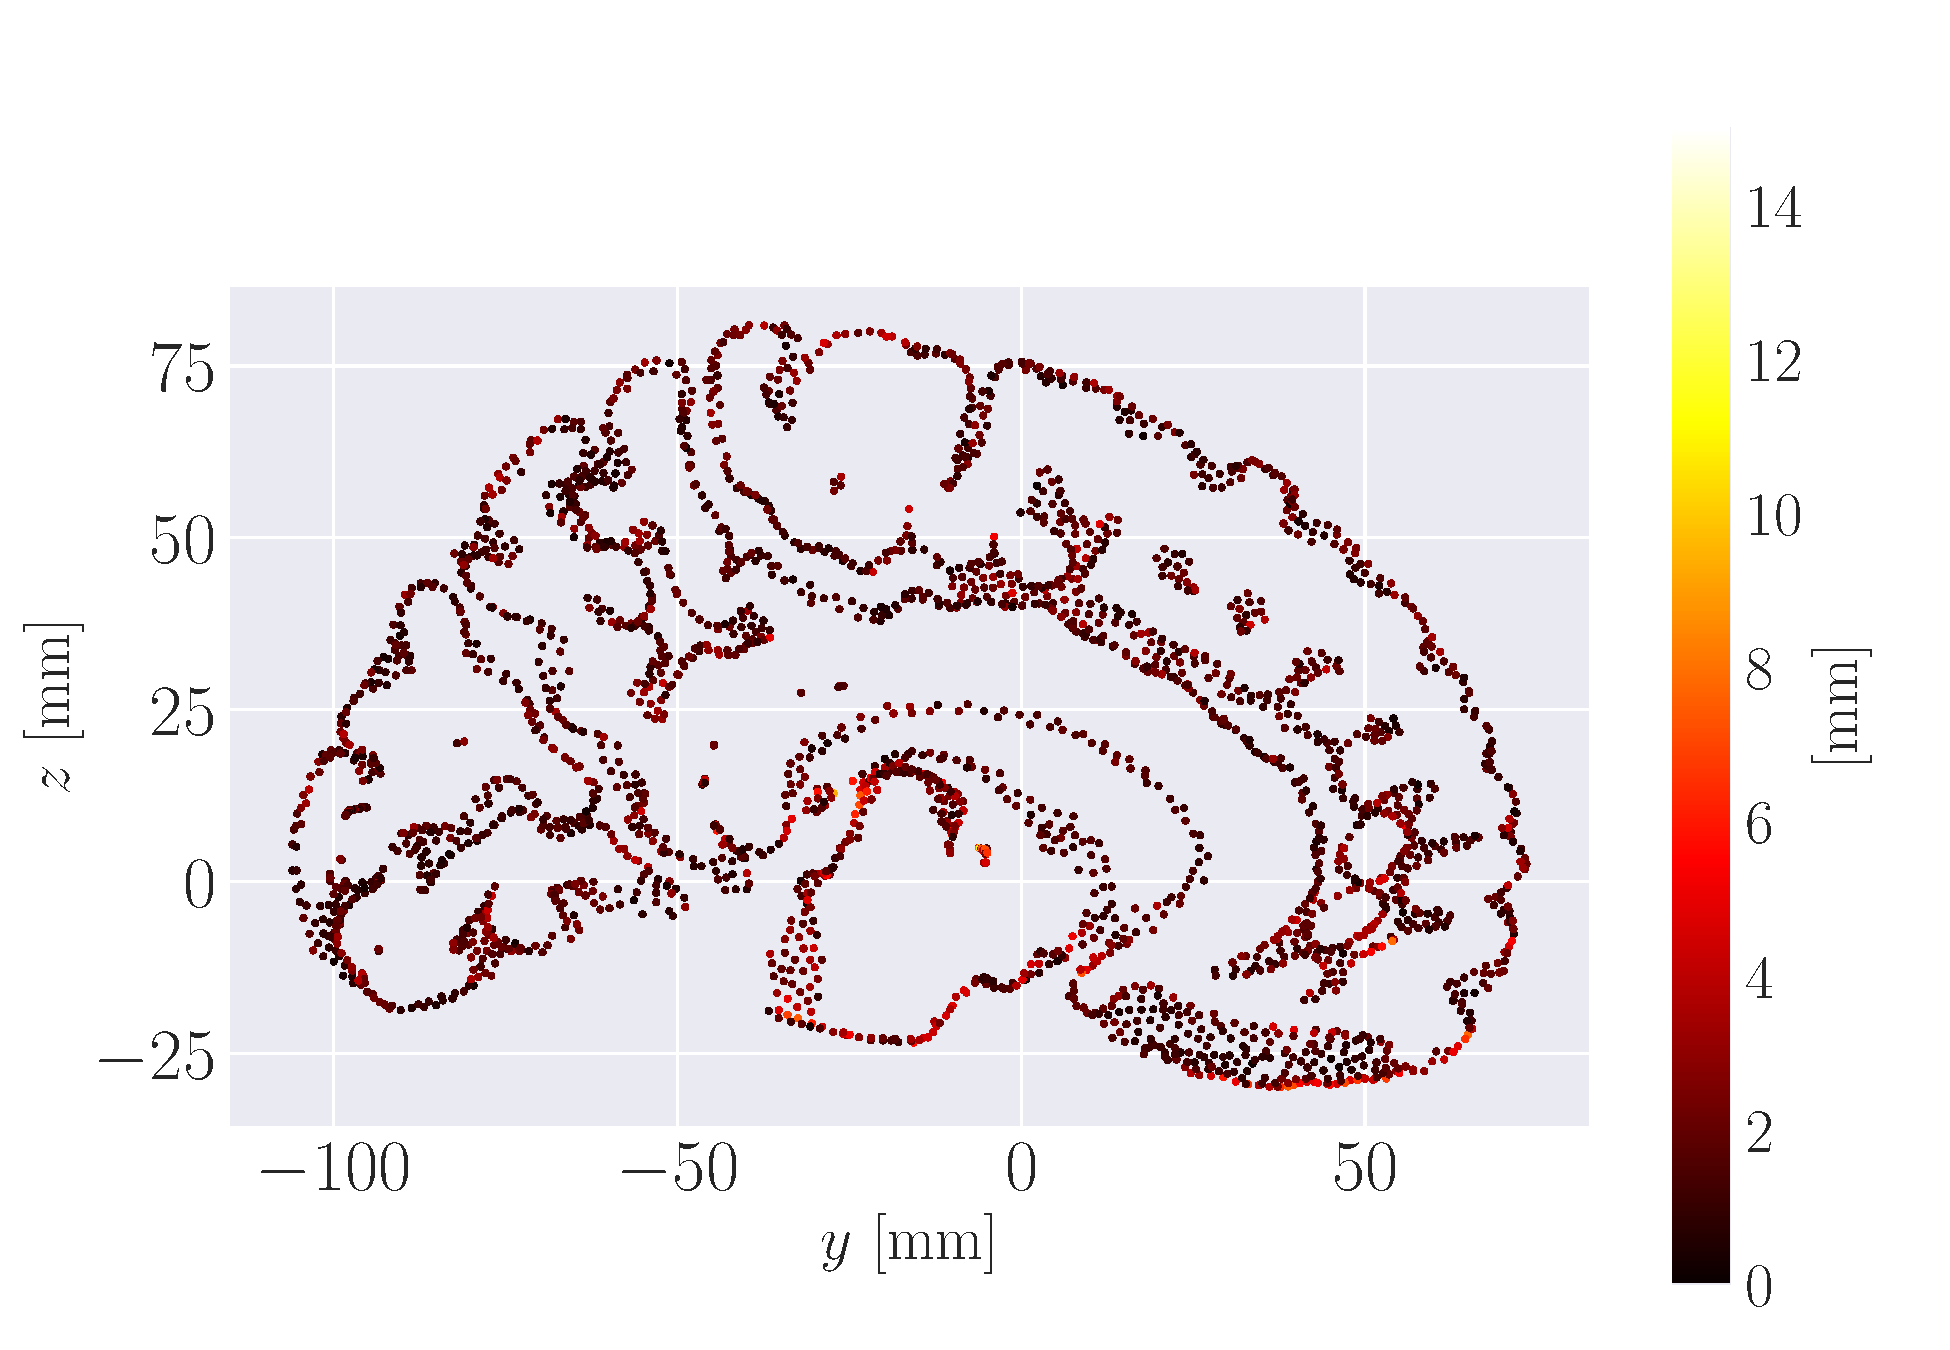
\includegraphics[width=1.0\textwidth]{figures/MED_simple_dipole_error_Euclidean Distance_2.pdf}
%       \end{itemize}
%     \end{column}
%   \end{columns}
% \end{frame}


% \begin{frame}{Convolutional Neural Network Approach I}
%     \begin{itemize}
%       \item[$\bullet$] Can spatial structures in EEG recordings enhance a neural network’s ability to analyze EEG data and yield more accurate predictions for localizing the sources generating the neural signals?
%       \item[$\bullet$] Convolutional Neural Networks are well-known for their effectiveness in processing image data.
%       \item[$\bullet$] Interpolate the original data set to create a input data resembling the structure of an image
%       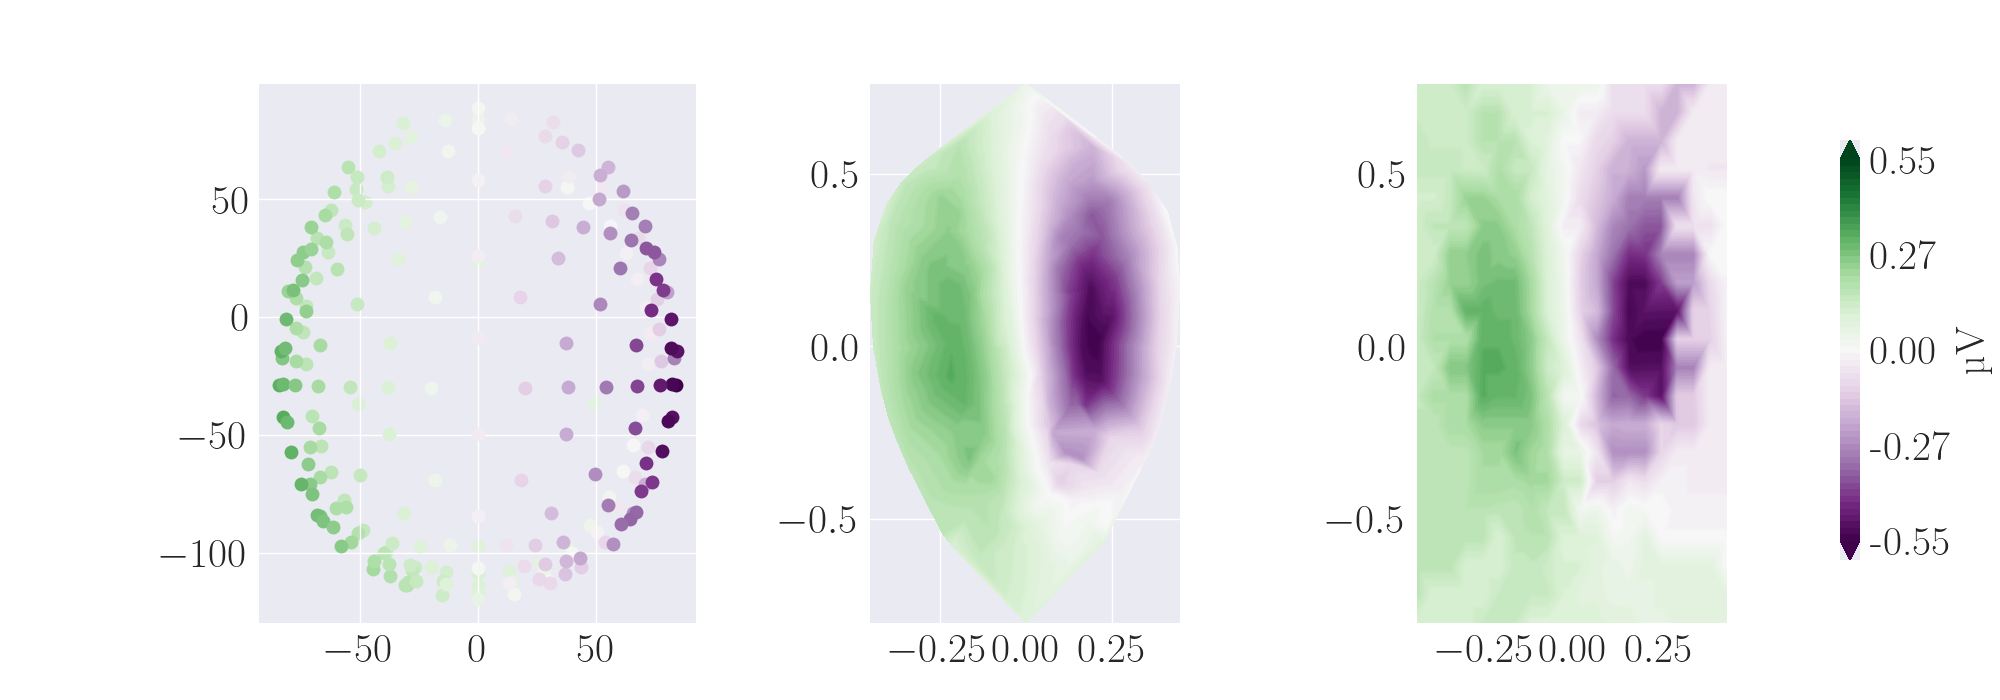
\includegraphics[width=0.8\textwidth]{figures/one_dipole_eeg_dipole_pos_0.png}
%     \end{itemize}
% \end{frame}
%
% \begin{frame}{Convolutional Neural Network Approach II}
%   \begin{columns}
%     \begin{column}{0.5\textwidth}
%       \begin{itemize}
%         \item[$\bullet$] Training time of 4 hours, 600 epochs
%         \item[$\bullet$] Training loss = 1.460 mm
%         \item[$\bullet$] Validation loss = 2.280 mm.
%         \item[$\bullet$] Test loss = 1.80 mm
%         \item[$\bullet$] Dipole located at $\tilde{x} = 66.5$ mm, $\tilde{y} = −26.5$ mm and $\tilde{z} = 41.9$ mm
%         \item[$\bullet$] Predicted $x = 66.4$ mm, $y = −27.3$ mm and $z = 41.5$ mm.
%         \item[$\bullet$] Euclidean distance = 0.99 mm.
%     \end{itemize}
%     \end{column}
%
%     \begin{column}{0.5\textwidth}
%       \begin{table}[]
%         \begin{tabular}{|ccc|}
%         \hline
%         \rowcolor[HTML]{CBCEFB}
%         \multicolumn{3}{|c|}{\cellcolor[HTML]{CBCEFB}\textbf{Euclidean Distance for Test Samples}}                                                             \\ \hline
%         \rowcolor[HTML]{EFEFEF}
%         \multicolumn{1}{|c|}{\cellcolor[HTML]{EFEFEF}ED \textless 5 mm} & \multicolumn{1}{c|}{\cellcolor[HTML]{EFEFEF}ED \textless 10 mm} & ED \textless 15 mm \\ \hline
%         \rowcolor[HTML]{FFFFFF}
%         \multicolumn{1}{|c|}{\cellcolor[HTML]{FFFFFF}98.030 $\%$}       & \multicolumn{1}{c|}{\cellcolor[HTML]{FFFFFF}99.815 $\%$}        & 99.993$\%$        \\ \hline
%         \end{tabular}
%       \end{table}
%     \end{column}
%
%   \end{columns}
% \end{frame}


\begin{frame}{Localizing Two Current Dipole Sources}
  \begin{columns}
    \begin{column}{0.5\textwidth}
      \begin{itemize}
        \item[$\bullet$] EEG data is modified to represent the electrical signals originating from two distinct dipoles, with positions $r_1$ and $r_2$, localized within the New York Head cortex.
        % \item[$\bullet$] The contibutions from the current dipole sources add up due to the linearity assumption.
        \item[$\bullet$] Six target values: $x_1, y_1, z_1, x_2, y_2, z_2$
        \item[$\bullet$] Customized cost function, checking for all possible permutations of target and prediction mappings (designed to accommodate an arbitrary number of dipoles)
    \end{itemize}
    \end{column}
    \begin{column}{0.5\textwidth}
    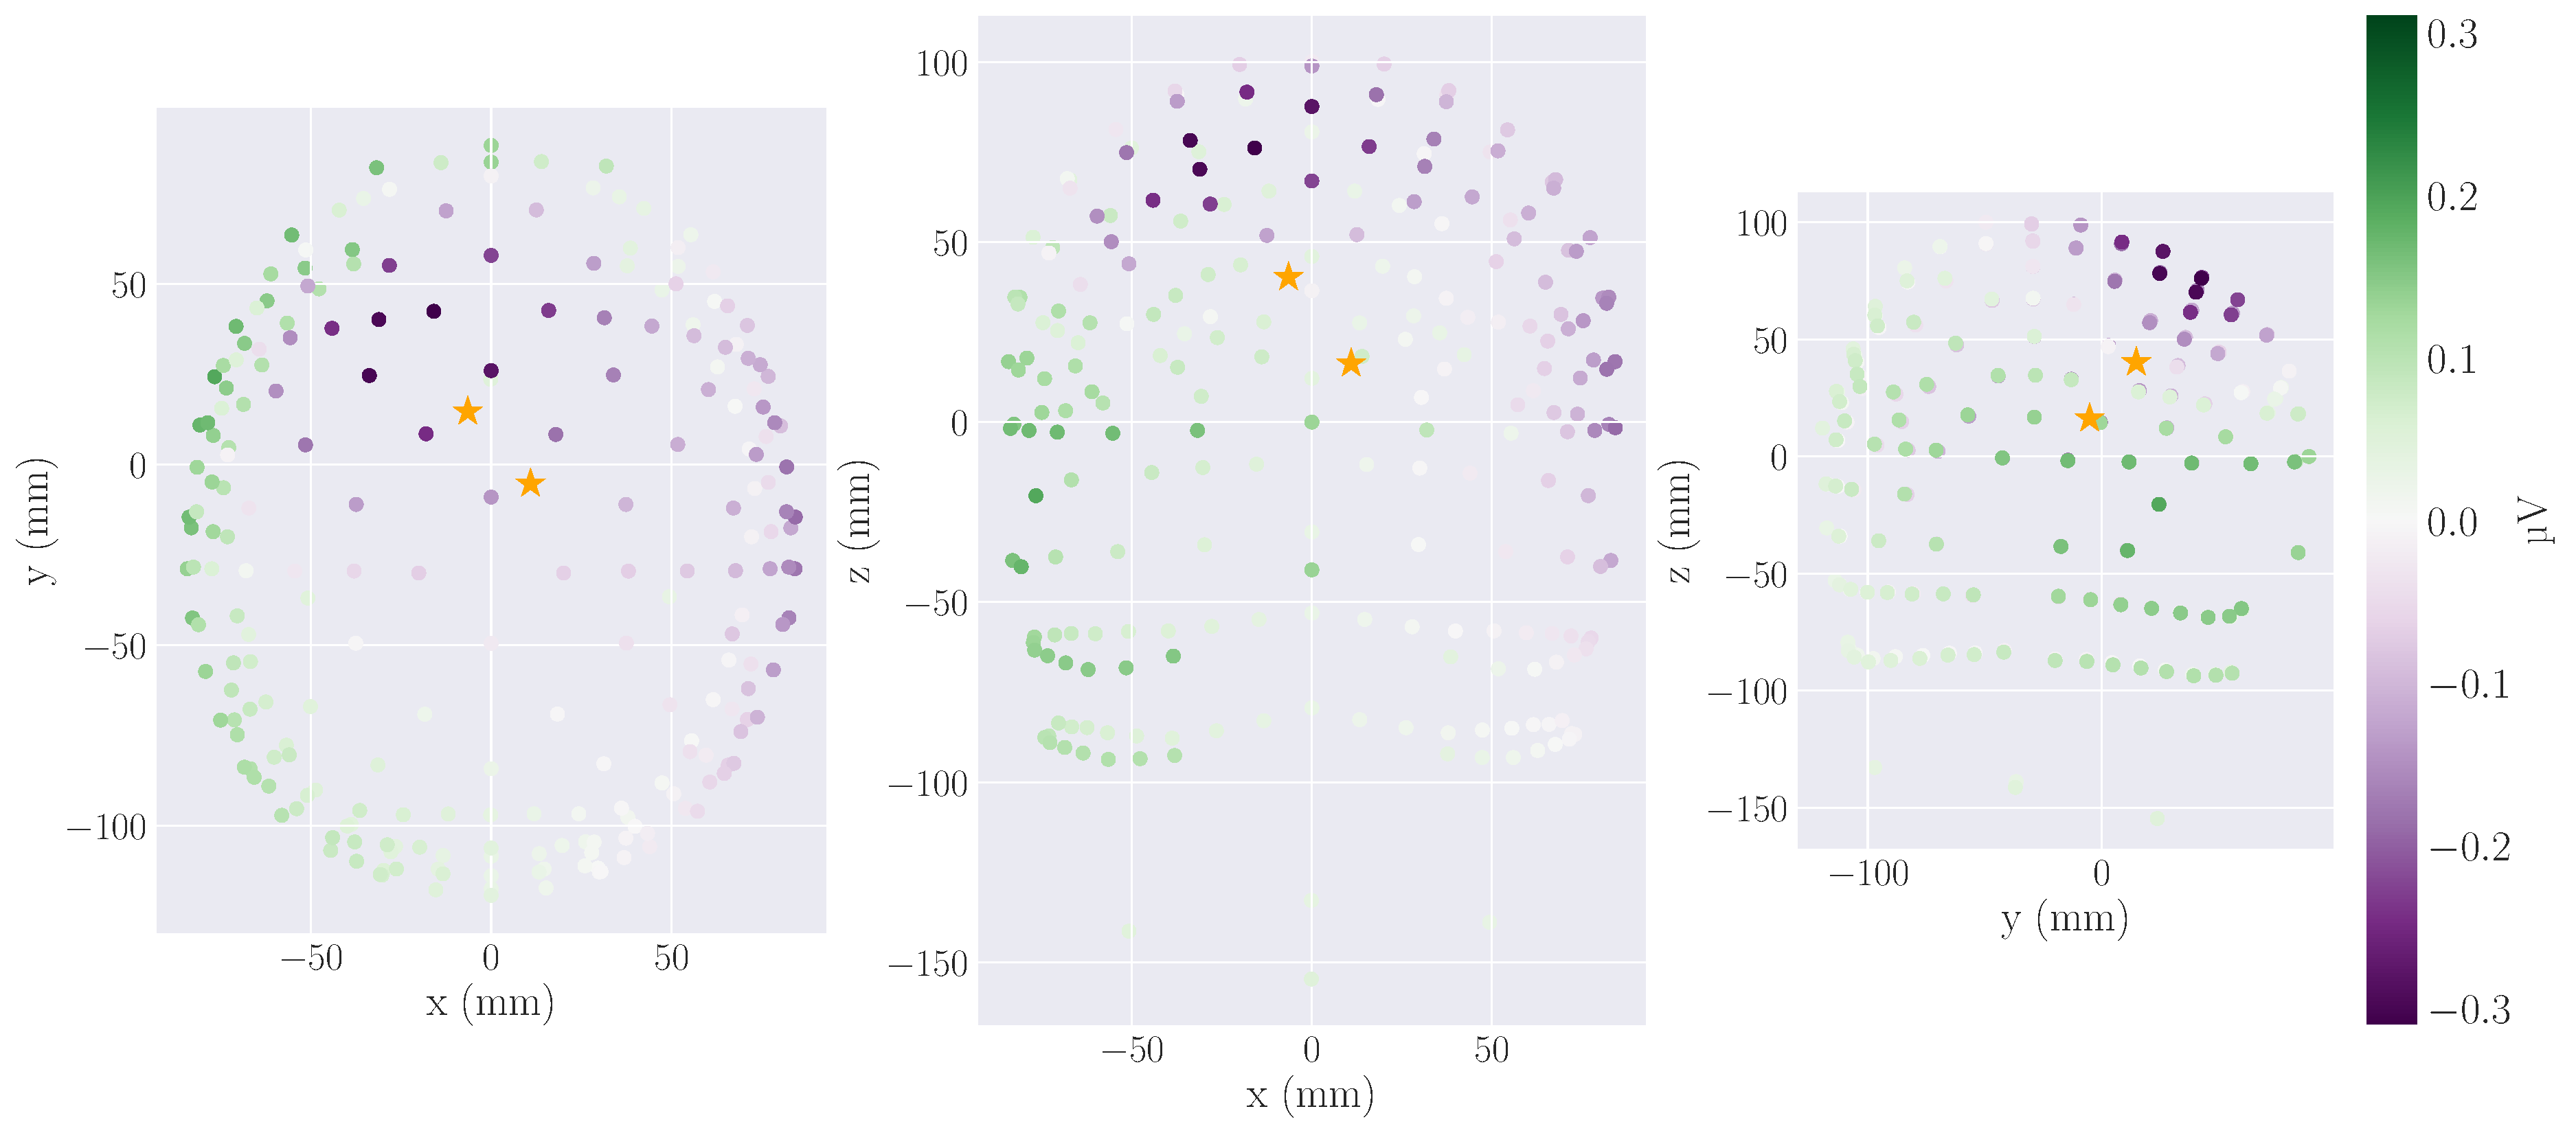
\includegraphics[width=7cm]{figures/dipoles_w_amplitudes_eeg_field_2_20.pdf}
    \end{column}
  \end{columns}
\end{frame}


\begin{frame}{Localizing Two Current Dipole Sources (FCNN)}
  \begin{columns}
    \begin{column}{0.5\textwidth}
      \begin{itemize}
        \item[$\bullet$] Training time of 6 hours, 800 epochs
        \item[$\bullet$] Validation loss: 9.36 mm
        \item[$\bullet$] Test loss: 8.71 mm
        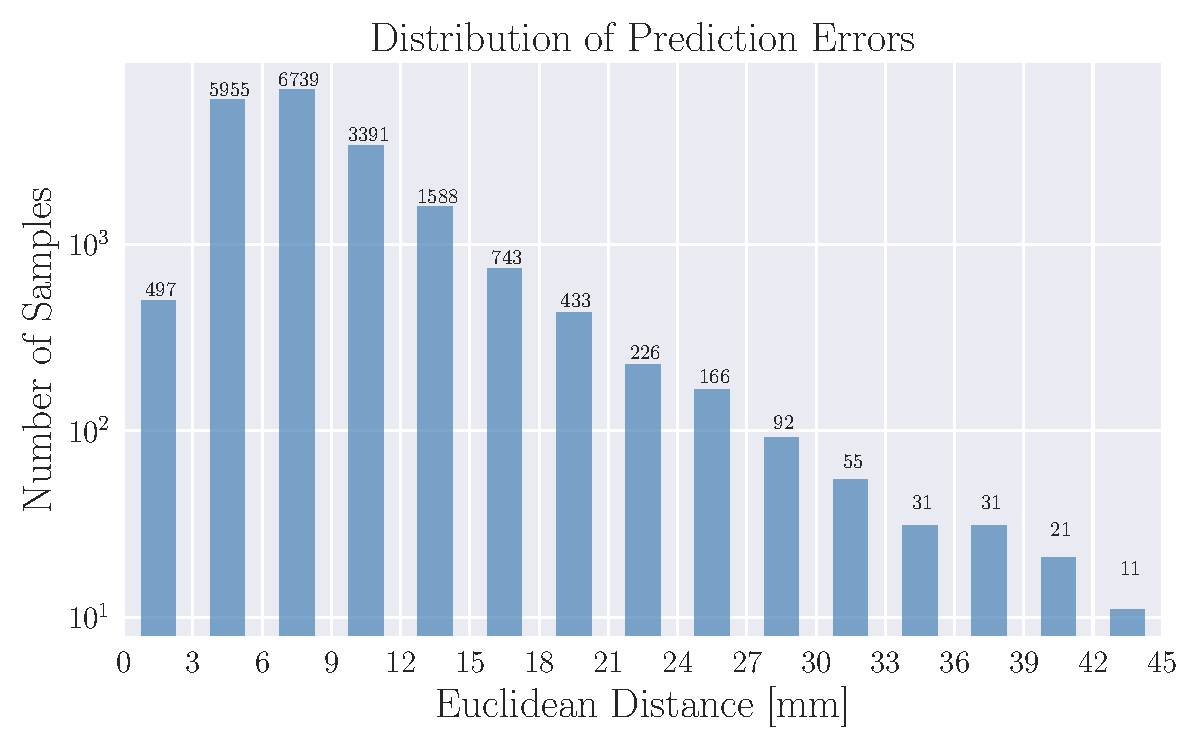
\includegraphics[width=6cm]{figures/new_histogram_2_dipoles_position_amplitude.pdf}
    \end{itemize}
    \end{column}
    \begin{column}{0.5\textwidth}
      % \begin{table}[]
      %   \begin{tabular}{|ccc|}
      %   \hline
      %   \rowcolor[HTML]{CBCEFB}
      %   \multicolumn{3}{|c|}{\cellcolor[HTML]{CBCEFB}\textbf{Euclidean Distance for Test Samples FCNN}}                                                             \\ \hline
      %   \rowcolor[HTML]{EFEFEF}
      %   \multicolumn{1}{|c|}{\cellcolor[HTML]{EFEFEF}ED \textless 5 mm} & \multicolumn{1}{c|}{\cellcolor[HTML]{EFEFEF}ED \textless 10 mm} & ED \textless 15 mm \\ \hline
      %   \rowcolor[HTML]{FFFFFF}
      %   \multicolumn{1}{|c|}{\cellcolor[HTML]{FFFFFF}18.995 $\%$}       & \multicolumn{1}{c|}{\cellcolor[HTML]{FFFFFF}73.055 $\%$}        & 90.850 $\%$        \\ \hline
      %   \end{tabular}
      % \end{table}
      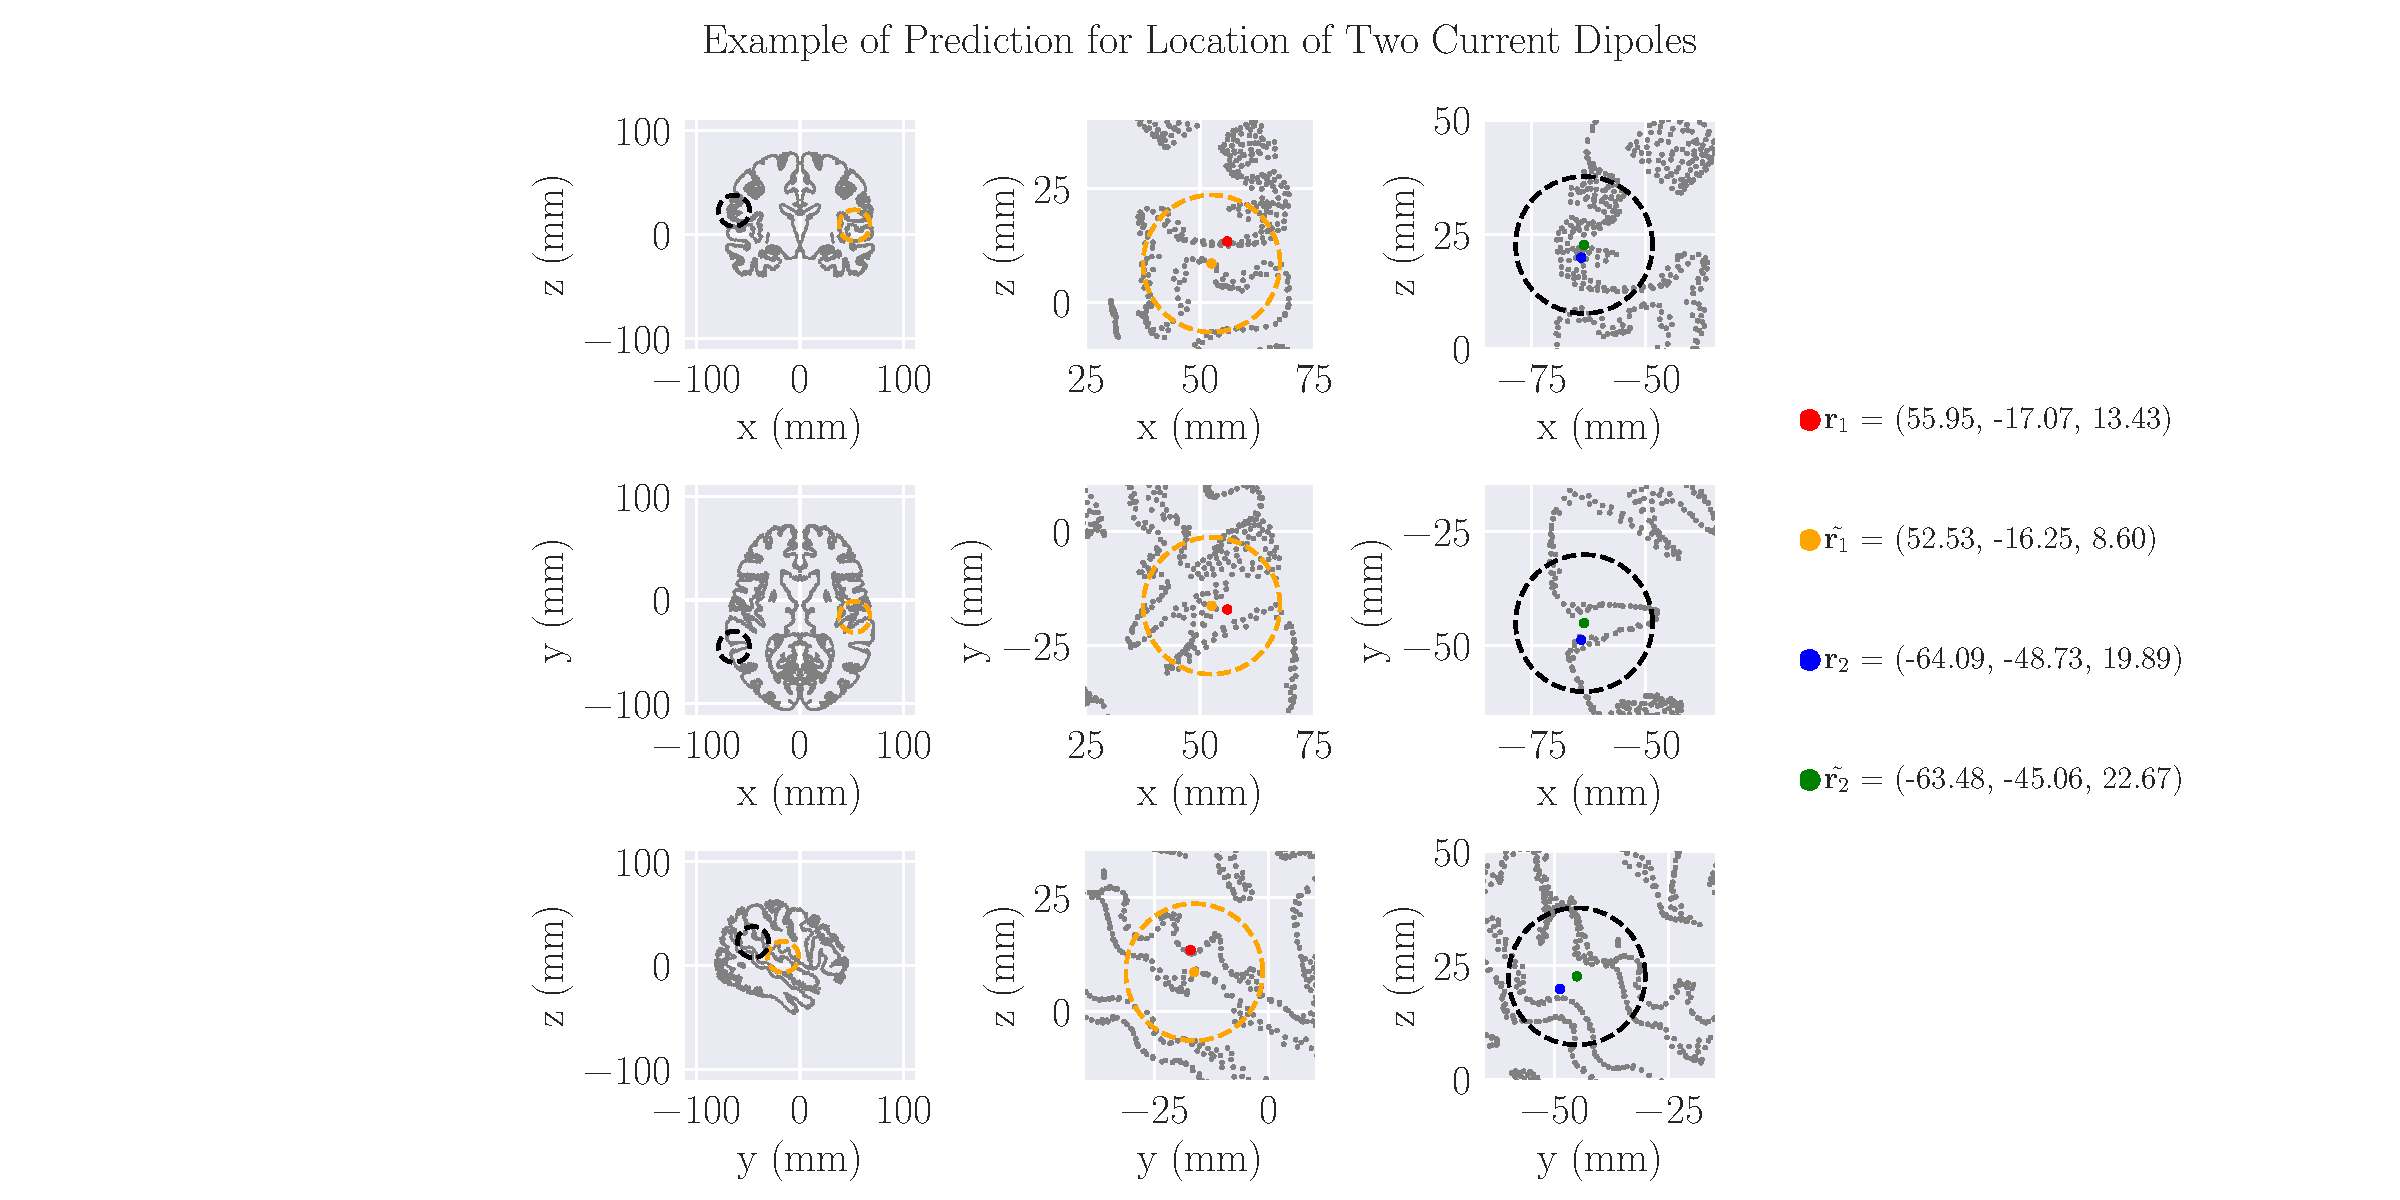
\includegraphics[width=7cm]{figures/two_dipoles_prediction.pdf}
      \begin{itemize}
      \item[$\bullet$] ED_{r_1} = 5.98 mm, ED_{r_1} = 4.65 mm
      \end{itemize}

    \end{column}
  \end{columns}
\end{frame}


% \begin{frame}{Localizing Two Current Dipole Sources (CNN)}
%   \begin{columns}
%     \begin{column}{0.5\textwidth}
%       \begin{itemize}
%         \item[$\bullet$] Training time of approximately 9 hours (NB: potential to be completed in half the time)
%         \item[$\bullet$] Validation loss: 9.83 mm
%         \item[$\bullet$] Test loss: 11.80 mm
%     \end{itemize}
%     \end{column}
%     \begin{column}{0.5\textwidth}
%       \begin{table}[]
%         \begin{tabular}{|ccc|}
%         \hline
%         \rowcolor[HTML]{CBCEFB}
%         \multicolumn{3}{|c|}{\cellcolor[HTML]{CBCEFB}\textbf{Euclidean Distance for Test Samples}}                                                             \\ \hline
%         \rowcolor[HTML]{EFEFEF}
%         \multicolumn{1}{|c|}{\cellcolor[HTML]{EFEFEF}ED \textless 5 mm} & \multicolumn{1}{c|}{\cellcolor[HTML]{EFEFEF}ED \textless 10 mm} & ED \textless 15 mm \\ \hline
%         \rowcolor[HTML]{FFFFFF}
%         \multicolumn{1}{|c|}{\cellcolor[HTML]{FFFFFF}7.545 $\%$}       & \multicolumn{1}{c|}{\cellcolor[HTML]{FFFFFF}50.460 $\%$}        & 78.870 $\%$        \\ \hline
%         \end{tabular}
%       \end{table}
%       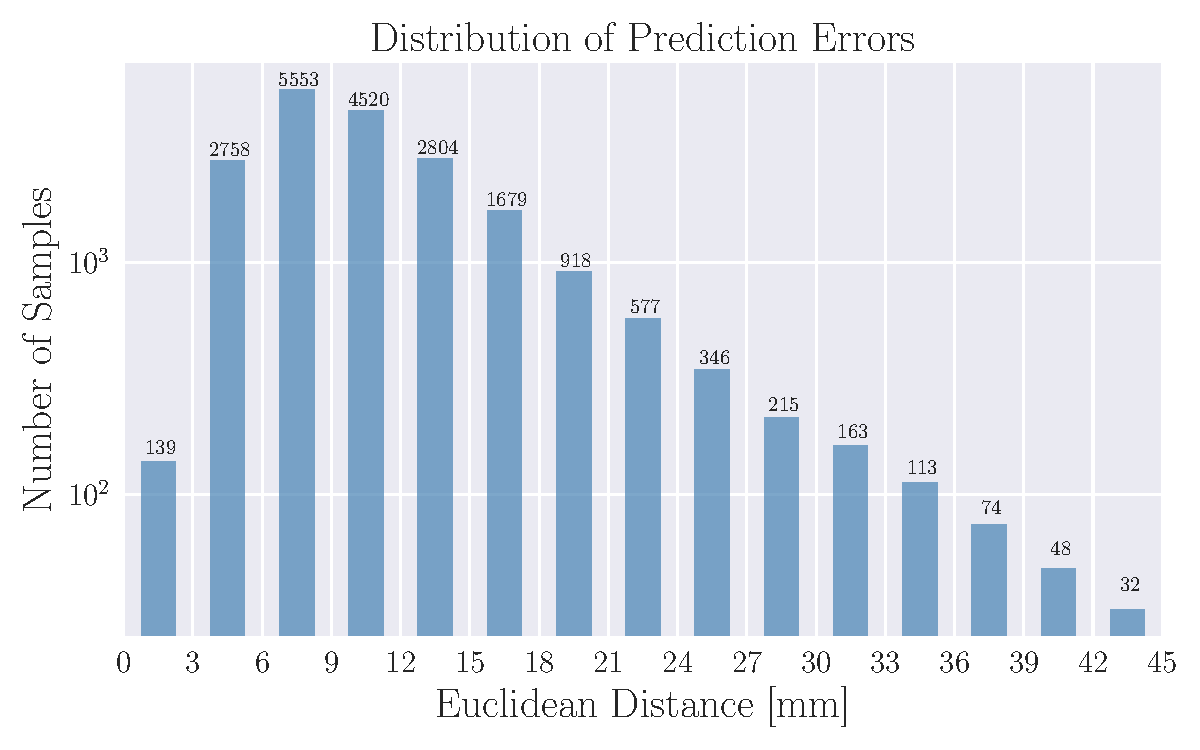
\includegraphics[width=7cm]{figures/new_histogram_2_dipoles_position_simple_cnn.pdf}
%
%     \end{column}
%   \end{columns}
% \end{frame}



\begin{frame}{Extending the FCNN}
  \begin{columns}
    \begin{column}{0.5\textwidth}
      \begin{itemize}
          \item[$\bullet$] Minor adjustments in data design and network architecture enhanced the FCNN’s ability to identify various attributes of current dipoles
          \begin{itemize}
            \item[\tiny$\blacksquare$] Predicting both location of the source and its corresponding magnitude.
            \item[\tiny$\blacksquare$] Estimate the center and radius of a population of dipoles, while also determining the magnitude of the signal strength of the entire dipole population.
          \end{itemize}
          \item[$\bullet$] Predicting target values that vary in range and units can result in a biased optimization process
          \item[$\bullet$] Normalizartion of the target data can address this issue
          \item[$\bullet$] With output ranging between 0 and 1, the Sigmoid activation function was utilized in the output layer, constraining the network from generating outputs beyond the intended normalized target range.
          \item[$\bullet$] Customized cost function combining the mean Euclidean distance for the position and mean absolute error for the magnitude and radius.
    \end{itemize}
    \end{column}
    \begin{column}{0.5\textwidth}
      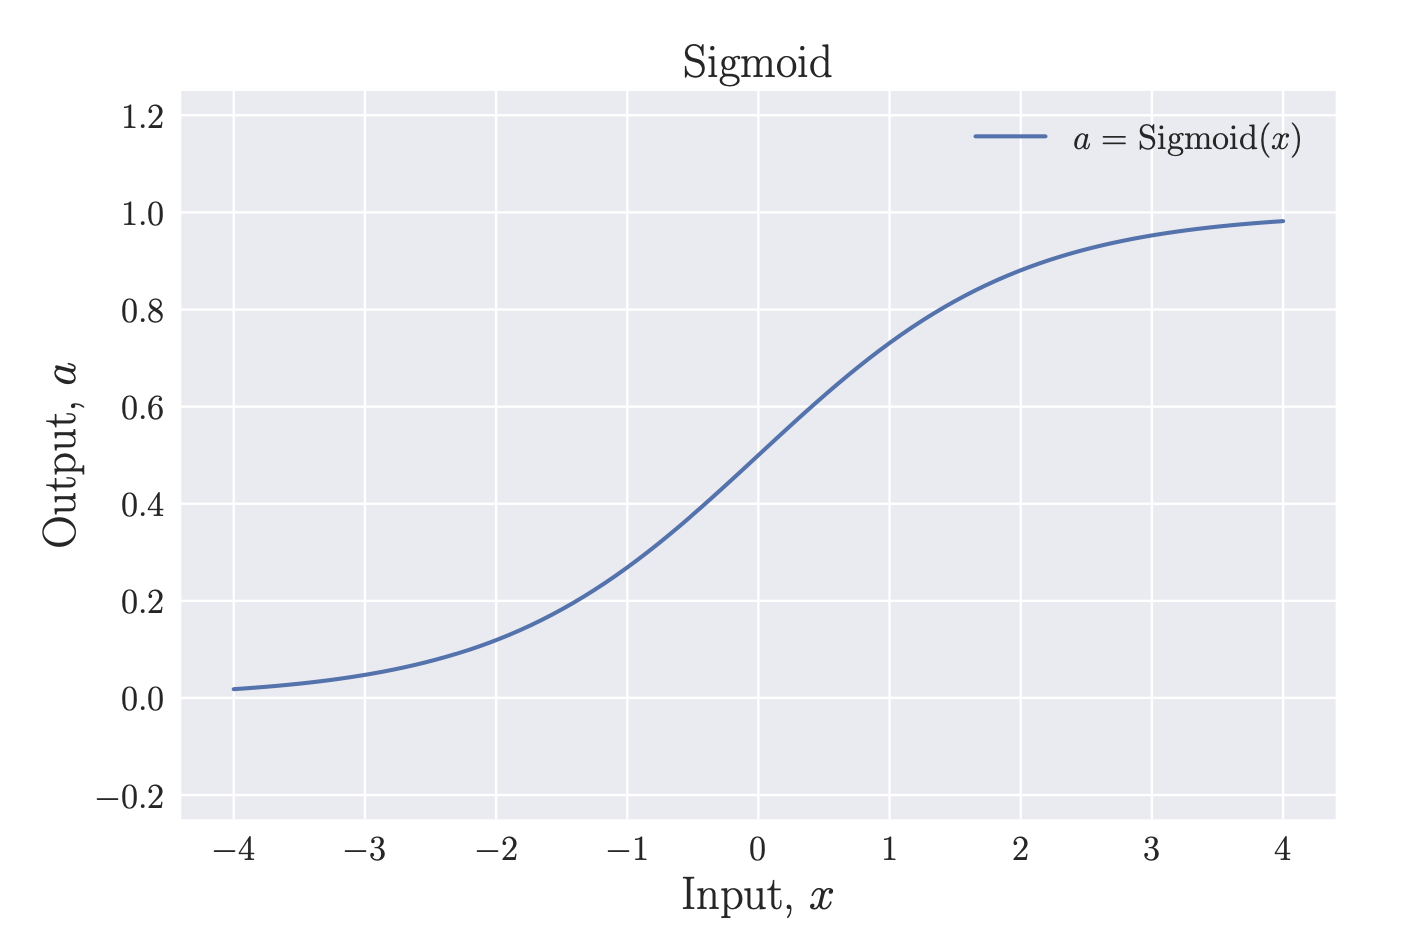
\includegraphics[width=7cm]{figures/sigmoid.png}
    \end{column}
  \end{columns}
\end{frame}



\begin{frame}{Predicting Single Current Dipole Sources with Varying Magnitudes}
  \begin{columns}
    \begin{column}{0.5\textwidth}
      \begin{itemize}
          \item[$\bullet$] Magnitude varying in strength from 1 to 10 nAm.
          \item[$\bullet$] 1500 training epochs gave a training time of $\sim$ 8.5 hours.

          \item[$\bullet$] Magnitude MAE = 0.539 nAm (6$\%$ of the magnitude range)
          \item[$\bullet$] MED = 2.82 mm
          % \begin{table}[]
          % \begin{tabular}{|ccc|}
          % \hline
          % \rowcolor[HTML]{CBCEFB}
          % \multicolumn{3}{|c|}{\cellcolor[HTML]{CBCEFB}\textbf{Euclidean Distance for Test Samples}}                                                             \\ \hline
          % \rowcolor[HTML]{EFEFEF}
          % \multicolumn{1}{|c|}{\cellcolor[HTML]{EFEFEF}ED \textless 5 mm} & \multicolumn{1}{c|}{\cellcolor[HTML]{EFEFEF}ED \textless 10 mm} & ED \textless 15 mm \\ \hline
          % \rowcolor[HTML]{FFFFFF}
          % \multicolumn{1}{|c|}{\cellcolor[HTML]{FFFFFF}90.930 $\%$}       & \multicolumn{1}{c|}{\cellcolor[HTML]{FFFFFF}99.505 $\%$}        & 99.925 $\%$        \\ \hline
          % \end{tabular}
          % \end{table}
    \end{itemize}
    \end{column}
    \begin{column}{0.5\textwidth}
      \vskip 0.5cm
      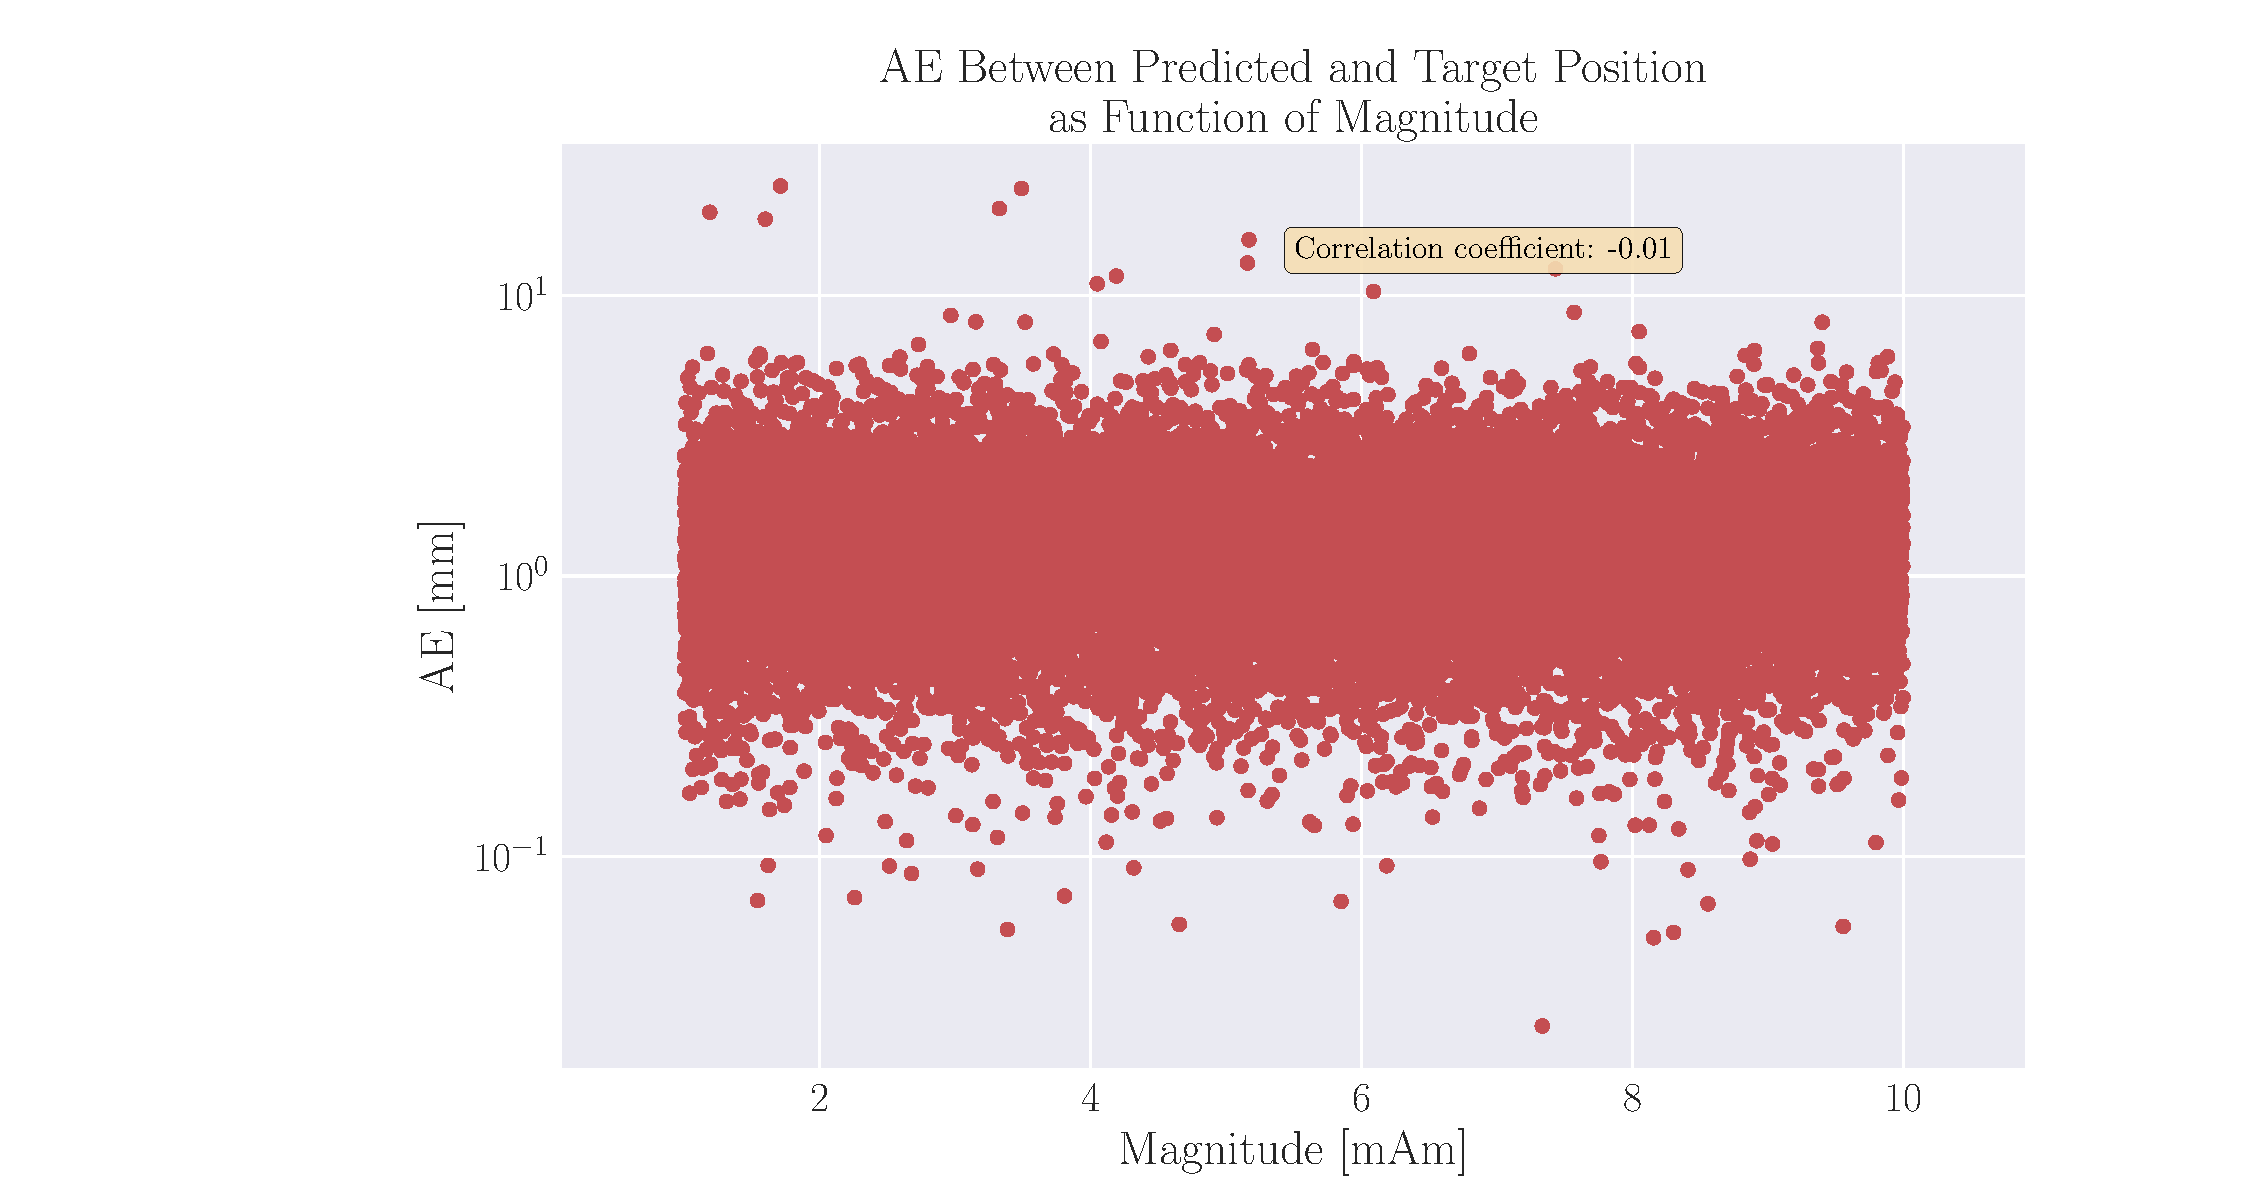
\includegraphics[width=7cm]{figures/mae_amplitude0.pdf}
    \end{column}
  \end{columns}
\end{frame}


\begin{frame}{Predicting Region of Active Correlated Current Dipoles with Magnitudes I}
        \begin{columns}
          \begin{column}{0.5\textwidth}
              \begin{itemize}
          \item[$\bullet$] Each dipole population comprises individual dipoles distributed across all points within the NY head cortex falling within a spherical volume ranging from 1 mm to 15 mm in radius.
          \item[$\bullet$] Maintain the maximum magnitude strength at 10 nAm.
          \item[$\bullet$] Maintained the maximum magnitude strength at 10 nAm. Consequently, the dipole strength for a distinct dipole was set to 10/899 nAm.
          \item[$\bullet$] Strength of dipole population directly proportional to the radius of the dipole population.
          \end{itemize}
          \end{column}
          \begin{column}{0.5\textwidth}
            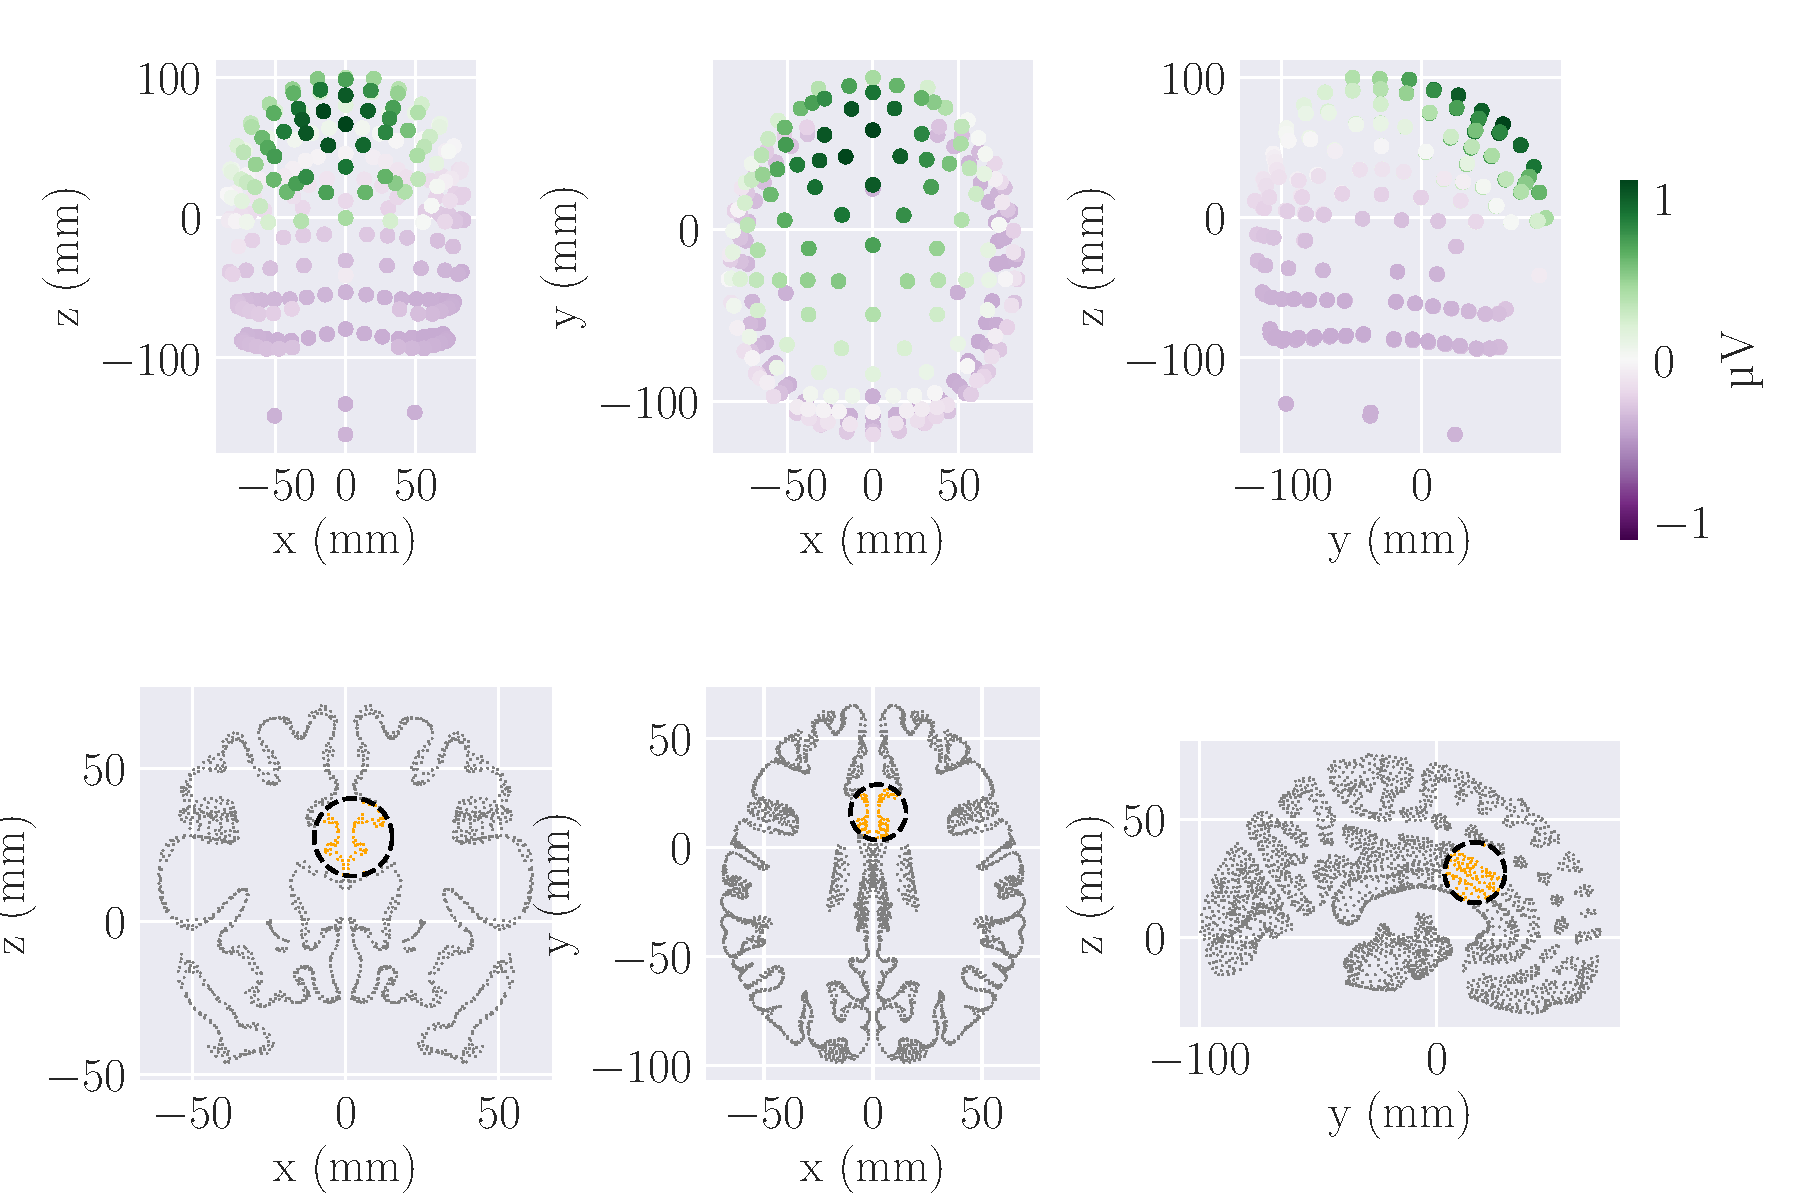
\includegraphics[width=7cm]{figures/dipole_area_reduced_0.pdf}
          \end{column}
          \end{columns}
%       \hspace*{10cm}
%       \begin{table}[]
%         \hspace*{-0.5cm}
%         \begin{tabular}{|ccc|l|ccc|l|ccc|}
%         \cline{1-3} \cline{5-7} \cline{9-11}
%         \multicolumn{3}{|c|}{\cellcolor[HTML]{CBCEFB}\textbf{Euclidean Distance: Position}}                                                                                                                                                                                                                             & \textbf{}             & \multicolumn{3}{c|}{\cellcolor[HTML]{CBCEFB}\textbf{Absolute Error: Magnitude}}                                                                                                                                                                                                                             & \textbf{}             & \multicolumn{3}{c|}{\cellcolor[HTML]{CBCEFB}\textbf{Absolute Error: Radius}}                                                                                                                                                                                                                                   \\ \cline{1-3} \cline{5-7} \cline{9-11}
%         \multicolumn{1}{|c|}{\cellcolor[HTML]{EFEFEF}\begin{tabular}[c]{@{}c@{}}ED \\ \textless 5 mm\end{tabular}} & \multicolumn{1}{c|}{\cellcolor[HTML]{EFEFEF}\begin{tabular}[c]{@{}c@{}}ED \\ \textless 10 mm\end{tabular}} & \cellcolor[HTML]{EFEFEF}\begin{tabular}[c]{@{}c@{}}ED \\ \textless 15 mm\end{tabular} &                       & \multicolumn{1}{c|}{\cellcolor[HTML]{EFEFEF}\begin{tabular}[c]{@{}c@{}}AE \\ \textless 1 nAm\end{tabular}} & \multicolumn{1}{c|}{\cellcolor[HTML]{EFEFEF}\begin{tabular}[c]{@{}c@{}}AE\\ \textless 2 nAm\end{tabular}} & \cellcolor[HTML]{EFEFEF}\begin{tabular}[c]{@{}c@{}}AE \\ \textless 3 nAm\end{tabular} &                       & \multicolumn{1}{c|}{\cellcolor[HTML]{EFEFEF}\begin{tabular}[c]{@{}c@{}}AE \\ \textless 1 mm\end{tabular}} & \multicolumn{1}{c|}{\cellcolor[HTML]{EFEFEF}\begin{tabular}[c]{@{}c@{}}AE \\ \textless 3 mm\end{tabular}} & \cellcolor[HTML]{EFEFEF}\begin{tabular}[c]{@{}c@{}}AE \\ \textless 5 mm\end{tabular} \\ \cline{1-3} \cline{5-7} \cline{9-11}
%         \multicolumn{1}{|c|}{56.045$\%$}                                                                           & \multicolumn{1}{c|}{79.680$\%$}                                                                            & 86.435$\%$                                                                            & \multicolumn{1}{c|}{} & \multicolumn{1}{c|}{92.900$\%$}                                                                           & \multicolumn{1}{c|}{98.565$\%$}                                                                          & 99.685$\%$                                                                           & \multicolumn{1}{c|}{} & \multicolumn{1}{c|}{74.210$\%$}                                                                           & \multicolumn{1}{c|}{98.220$\%$}                                                                            & 99.770$\%$                                                                            \\ \cline{1-3} \cline{5-7} \cline{9-11}
%       \end{tabular}
% \end{table}

\end{frame}


\begin{frame}{Predicting Region of Active Correlated Current Dipoles with Magnitudes II}
  \begin{columns}
    \begin{column}{0.5\textwidth}
      \begin{itemize}
      \item[$\bullet$] 1000 training epochs gave a training time of $\sim$ 9.5 hours.
      \item[$\bullet$] Radius MAE = 0.76 mm (5.4$\%$ of the radius range)
      \item[$\bullet$] Magnitude MAE = 0.33 nAm (3.7$\%$ of the magnitude range)
      \item[$\bullet$] MED = 7.85 mm
    \end{itemize}
    \end{column}
    \begin{column}{0.5\textwidth}
      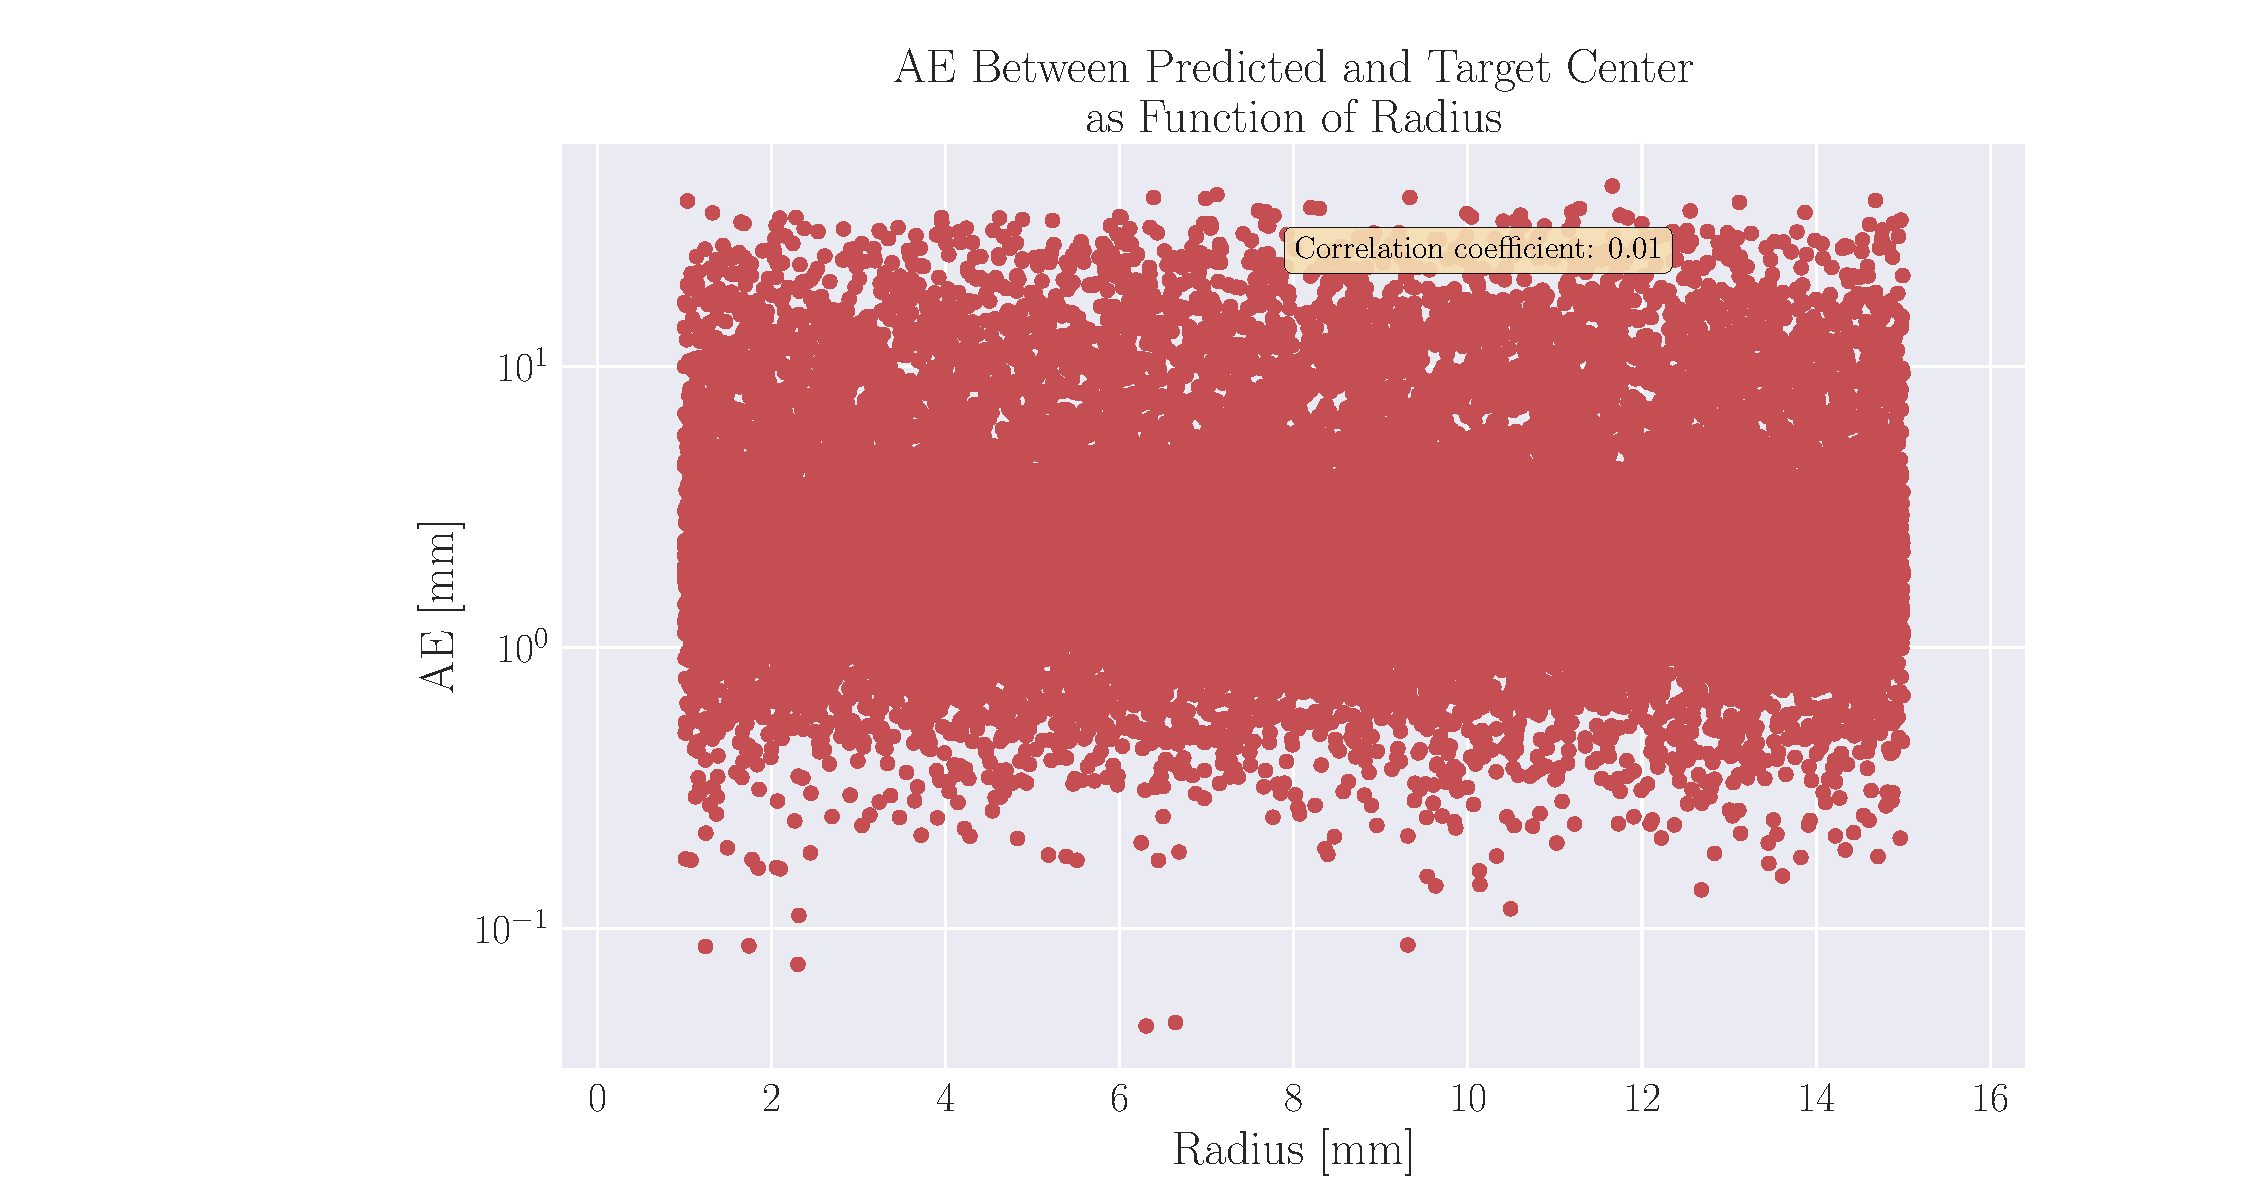
\includegraphics[width=7cm]{figures/mae_area.pdf}
    \end{column}
  \end{columns}
\end{frame}


%    \begin{table}[]
% \hspace*{-0.5cm} % Adjust the value as needed to move the figures left
% \begin{tabular}{c|cccccc|}
% \cline{2-7}
% \multicolumn{1}{l|}{}                                                                                               & \multicolumn{6}{c|}{\cellcolor[HTML]{CBCEFB}\textbf{Summary of Main Results}}                                                                                                                                                                                                                                                                                                                                                                                                                                                                                                                                                                                      \\ \cline{2-7}
% \multicolumn{1}{l|}{}                                                                                               & \multicolumn{1}{c|}{\cellcolor[HTML]{EFEFEF}\begin{tabular}[c]{@{}c@{}}Singe Dipole:\\ FCNN\end{tabular}} & \multicolumn{1}{c|}{\cellcolor[HTML]{EFEFEF}\begin{tabular}[c]{@{}c@{}}Single Dipoles:\\ CNN\end{tabular}} & \multicolumn{1}{c|}{\cellcolor[HTML]{EFEFEF}\begin{tabular}[c]{@{}c@{}}Two Dipoles:\\ FCNN\end{tabular}} & \multicolumn{1}{c|}{\cellcolor[HTML]{EFEFEF}\begin{tabular}[c]{@{}c@{}}Two Dipoles:\\ CNN\end{tabular}} & \multicolumn{1}{c|}{\cellcolor[HTML]{EFEFEF}\begin{tabular}[c]{@{}c@{}}Dipole with \\ Magnitude:\\ FCNN\end{tabular}} & \cellcolor[HTML]{EFEFEF}\begin{tabular}[c]{@{}c@{}}Dipole \\ Population:\\ FCNN\end{tabular} \\ \hline
% \multicolumn{1}{|c|}{\cellcolor[HTML]{EFEFEF}$d$}                                                                   & \multicolumn{1}{c|}{3}                                                                                    & \multicolumn{1}{c|}{3}                                                                                     & \multicolumn{1}{c|}{6}                                                                                   & \multicolumn{1}{c|}{6}                                                                                  & \multicolumn{1}{c|}{4}                                                                                                & 5                                                                                            \\ \hline
% \multicolumn{1}{|c|}{\cellcolor[HTML]{EFEFEF}\begin{tabular}[c]{@{}c@{}}Coordinate with\\ highest MAE\end{tabular}} & \multicolumn{1}{c|}{z}                                                                                    & \multicolumn{1}{c|}{z}                                                                                     & \multicolumn{1}{c|}{z}                                                                                   & \multicolumn{1}{c|}{z}                                                                                  & \multicolumn{1}{c|}{y}                                                                                                & z                                                                                            \\ \hline
% \multicolumn{1}{|c|}{\cellcolor[HTML]{EFEFEF}MED($x, y, z$) {[}mm{]}}                                               & \multicolumn{1}{c|}{1.3}                                                                                  & \multicolumn{1}{c|}{1.8}                                                                                   & \multicolumn{1}{c|}{8.71}                                                                                & \multicolumn{1}{c|}{11.78}                                                                              & \multicolumn{1}{c|}{2.815}                                                                                            & 7.85                                                                                         \\ \hline
% \multicolumn{1}{|c|}{\cellcolor[HTML]{EFEFEF}MSE($x, y, z$) {[}mm$^2${]}}                                           & \multicolumn{1}{c|}{0.782}                                                                                & \multicolumn{1}{c|}{1.643}                                                                                 & \multicolumn{1}{c|}{38.978}                                                                              & \multicolumn{1}{c|}{69.306}                                                                             & \multicolumn{1}{c|}{3.720}                                                                                            & 50.359                                                                                       \\ \hline
% \multicolumn{1}{|c|}{\cellcolor[HTML]{EFEFEF}MAE($x, y, z$) {[}mm{]}}                                               & \multicolumn{1}{c|}{0.662}                                                                                & \multicolumn{1}{c|}{0.898}                                                                                 & \multicolumn{1}{c|}{4.340}                                                                               & \multicolumn{1}{c|}{5.731}                                                                              & \multicolumn{1}{c|}{1.405}                                                                                            & 3.961                                                                                        \\ \hline
% \multicolumn{1}{|c|}{\cellcolor[HTML]{EFEFEF}MAE$_A$ {[}nAm{]}}                                                 & \multicolumn{1}{c|}{-}                                                                                    & \multicolumn{1}{c|}{-}                                                                                     & \multicolumn{1}{c|}{-}                                                                                   & \multicolumn{1}{c|}{-}                                                                                  & \multicolumn{1}{c|}{0.539}                                                                                            & 0.33                                                                                         \\ \hline
% \multicolumn{1}{|c|}{\cellcolor[HTML]{EFEFEF}MAE$_R$ {[}mm{]}}                                                      & \multicolumn{1}{c|}{-}                                                                                    & \multicolumn{1}{c|}{-}                                                                                     & \multicolumn{1}{c|}{-}                                                                                   & \multicolumn{1}{c|}{-}                                                                                  & \multicolumn{1}{c|}{-}                                                                                                & 0.76                                                                                         \\ \hline
% \end{tabular}
% \caption{Summary of main results of the thesis.}
% \label{table:sum_main_results}
% \end{table}
% \end{frame}
%

\begin{frame}{Positional Errors}
    \begin{itemize}
      % \item[$\bullet$] A slightly higher MAE was observed in the $z$-coordinate.
      % \item[$\bullet$] Recording electrodes are situated along both the right-left and front-back directions, whereas electrodes along the z-axis are primarily placed on top of the head.
      \item[$\bullet$] Modern subject-specific head models is expected to result in mean Euclidean errors less than 10 mm (Akalin and Makeig 2013, Biasiucci et al. 2019).
      \item[$\bullet$] In most of our approaches we successfully achived localization errors smaller than the 10 mm threshold.
      \item[$\bullet$] In clinical contexts, there exists a considerable difference between errors below this value.
      \item[$\bullet$] An error of 1.3 mm, as observed in the case of the FCNN predicting dipole position alone, is significantly more accurate than the 8.71 mm error observed when predicting the position of two current dipoles.
      \item[$\bullet$] Essential to recognize that minimizing the error beyond a certain point not necessarily result in substantial clinical advantages.
    \end{itemize}
\end{frame}

\begin{frame}{Predicting Dipole Strength and Population Radius}
    \begin{itemize}
      \item[$\bullet$] Inherent correlation between the prediction of radius and strength.
      \item[$\bullet$] When predicting both magnitude and radius, the optimizartion process indirectly give more importance to reducing errors according to these values.
      \item[$\bullet$] This correlation lead to improvent in MAE$_{\text{A}}$ in comparison to when only predicting magnitude.
    \end{itemize}
\end{frame}

% \begin{frame}{Data}
%     \begin{itemize}
%       \item[$\bullet$] Self-simulated data provides high degree of control.
%       \item[$\bullet$] The extent to which our networks faithfully capture the complexity, noise, and variability present in clinical EEG data will not align with the performance demonstrated on simulated validation and test data.
%       \item[$\bullet$] Can expect suboptimal performance if directly applied to EEG recordings from real patients.
%     \end{itemize}
% \end{frame}


\begin{frame}{Computational Speed}
    \begin{itemize}
      \item[$\bullet$] 1 - 9 hours, depending on the network complexity.
      \item[$\bullet$] The networks exhibit efficient execution times for individual samples once trained.
      \item[$\bullet$] Plausible to construct patient-specific head models that can be integrated into our framework, subsequently training the networks with data extracted from the patients head models.
      \item[$\bullet$] Head-specific models would require time to develop -- but once fully trained, likely to require very short time for outputting predictions.
      % \item[$\bullet$] Neural networks are potentially invaluable tools in clinical applications of EEG.
    \end{itemize}
\end{frame}


% \begin{frame}{Conclusion}
%     \begin{itemize}
%     \end{itemize}
% \end{frame}


\end{document}
